% Options for packages loaded elsewhere
% Options for packages loaded elsewhere
\PassOptionsToPackage{unicode}{hyperref}
\PassOptionsToPackage{hyphens}{url}
\PassOptionsToPackage{dvipsnames,svgnames,x11names}{xcolor}
%
\documentclass[
  english,
  11pt,
  letterpaper,
]{article}
\usepackage{xcolor}
\usepackage[margin=1in]{geometry}
\usepackage{amsmath,amssymb}
\setcounter{secnumdepth}{5}
\usepackage{iftex}
\ifPDFTeX
  \usepackage[T1]{fontenc}
  \usepackage[utf8]{inputenc}
  \usepackage{textcomp} % provide euro and other symbols
\else % if luatex or xetex
  \usepackage{unicode-math} % this also loads fontspec
  \defaultfontfeatures{Scale=MatchLowercase}
  \defaultfontfeatures[\rmfamily]{Ligatures=TeX,Scale=1}
\fi
\usepackage{lmodern}
\ifPDFTeX\else
  % xetex/luatex font selection
\fi
% Use upquote if available, for straight quotes in verbatim environments
\IfFileExists{upquote.sty}{\usepackage{upquote}}{}
\IfFileExists{microtype.sty}{% use microtype if available
  \usepackage[]{microtype}
  \UseMicrotypeSet[protrusion]{basicmath} % disable protrusion for tt fonts
}{}
\makeatletter
\@ifundefined{KOMAClassName}{% if non-KOMA class
  \IfFileExists{parskip.sty}{%
    \usepackage{parskip}
  }{% else
    \setlength{\parindent}{0pt}
    \setlength{\parskip}{6pt plus 2pt minus 1pt}}
}{% if KOMA class
  \KOMAoptions{parskip=half}}
\makeatother
% Make \paragraph and \subparagraph free-standing
\makeatletter
\ifx\paragraph\undefined\else
  \let\oldparagraph\paragraph
  \renewcommand{\paragraph}{
    \@ifstar
      \xxxParagraphStar
      \xxxParagraphNoStar
  }
  \newcommand{\xxxParagraphStar}[1]{\oldparagraph*{#1}\mbox{}}
  \newcommand{\xxxParagraphNoStar}[1]{\oldparagraph{#1}\mbox{}}
\fi
\ifx\subparagraph\undefined\else
  \let\oldsubparagraph\subparagraph
  \renewcommand{\subparagraph}{
    \@ifstar
      \xxxSubParagraphStar
      \xxxSubParagraphNoStar
  }
  \newcommand{\xxxSubParagraphStar}[1]{\oldsubparagraph*{#1}\mbox{}}
  \newcommand{\xxxSubParagraphNoStar}[1]{\oldsubparagraph{#1}\mbox{}}
\fi
\makeatother


\usepackage{longtable,booktabs,array}
\newcounter{none} % for unnumbered tables
\usepackage{calc} % for calculating minipage widths
% Correct order of tables after \paragraph or \subparagraph
\usepackage{etoolbox}
\makeatletter
\patchcmd\longtable{\par}{\if@noskipsec\mbox{}\fi\par}{}{}
\makeatother
% Allow footnotes in longtable head/foot
\IfFileExists{footnotehyper.sty}{\usepackage{footnotehyper}}{\usepackage{footnote}}
\makesavenoteenv{longtable}
\usepackage{graphicx}
\makeatletter
\newsavebox\pandoc@box
\newcommand*\pandocbounded[1]{% scales image to fit in text height/width
  \sbox\pandoc@box{#1}%
  \Gscale@div\@tempa{\textheight}{\dimexpr\ht\pandoc@box+\dp\pandoc@box\relax}%
  \Gscale@div\@tempb{\linewidth}{\wd\pandoc@box}%
  \ifdim\@tempb\p@<\@tempa\p@\let\@tempa\@tempb\fi% select the smaller of both
  \ifdim\@tempa\p@<\p@\scalebox{\@tempa}{\usebox\pandoc@box}%
  \else\usebox{\pandoc@box}%
  \fi%
}
% Set default figure placement to htbp
\def\fps@figure{htbp}
\makeatother



\ifLuaTeX
\usepackage[bidi=basic,shorthands=off]{babel}
\else
\usepackage[bidi=default,shorthands=off]{babel}
\fi
\ifLuaTeX
  \usepackage{selnolig} % disable illegal ligatures
\fi


\setlength{\emergencystretch}{3em} % prevent overfull lines

\providecommand{\tightlist}{%
  \setlength{\itemsep}{0pt}\setlength{\parskip}{0pt}}



 


\makeatletter
\@ifpackageloaded{caption}{}{\usepackage{caption}}
\AtBeginDocument{%
\ifdefined\contentsname
  \renewcommand*\contentsname{Table of contents}
\else
  \newcommand\contentsname{Table of contents}
\fi
\ifdefined\listfigurename
  \renewcommand*\listfigurename{List of Figures}
\else
  \newcommand\listfigurename{List of Figures}
\fi
\ifdefined\listtablename
  \renewcommand*\listtablename{List of Tables}
\else
  \newcommand\listtablename{List of Tables}
\fi
\ifdefined\figurename
  \renewcommand*\figurename{Figure}
\else
  \newcommand\figurename{Figure}
\fi
\ifdefined\tablename
  \renewcommand*\tablename{Table}
\else
  \newcommand\tablename{Table}
\fi
}
\@ifpackageloaded{float}{}{\usepackage{float}}
\floatstyle{ruled}
\@ifundefined{c@chapter}{\newfloat{codelisting}{h}{lop}}{\newfloat{codelisting}{h}{lop}[chapter]}
\floatname{codelisting}{Listing}
\newcommand*\listoflistings{\listof{codelisting}{List of Listings}}
\makeatother
\makeatletter
\makeatother
\makeatletter
\@ifpackageloaded{caption}{}{\usepackage{caption}}
\@ifpackageloaded{subcaption}{}{\usepackage{subcaption}}
\makeatother
\usepackage{bookmark}
\IfFileExists{xurl.sty}{\usepackage{xurl}}{} % add URL line breaks if available
\urlstyle{same}
% fallback for those not using the hyperref driver hyperxmp:
\makeatletter
\@ifundefined{xmpquote}{\newcommand{\xmpquote}[1]{#1}}{}
\makeatother
\hypersetup{
  pdftitle={Scalable Fraud Detection in Banking Chatbot Conversations},
  pdfauthor={Mingyang Han; Yuhua Pang; Zhaoyang Dong; Wenhao Zhou},
  pdflang={en},
  colorlinks=true,
  linkcolor={blue},
  filecolor={Maroon},
  citecolor={Blue},
  urlcolor={Blue},
  pdfcreator={LaTeX via pandoc}}


\title{Scalable Fraud Detection in Banking Chatbot Conversations}
\usepackage{etoolbox}
\makeatletter
\providecommand{\subtitle}[1]{% add subtitle to \maketitle
  \apptocmd{\@title}{\par {\large #1 \par}}{}{}
}
\makeatother
\subtitle{DSAN 6000 Final Project}
\author{Mingyang Han \and Yuhua Pang \and Zhaoyang Dong \and Wenhao
Zhou}
\date{}
\begin{document}
\maketitle
\begin{abstract}
This project aims to detect fraud messages in conversations with a bank
chatbot. We use the Banking77 dataset from PolyAI, which contains 13,083
customer messages labeled with 77 intents, together with a message
stream simulated from its training split. An extract, transform, and
load (ETL) process cleans the text, builds an intent catalog, and stores
date-partitioned Parquet data for processing in Amazon S3 and Apache
Spark. We use natural language processing and machine learning to
classify message intent and investigate text and behavior signals for
fraud detection. The completed experiments achieve 89.06\% intent
accuracy with a scikit-learn model and 84.45\% with a Spark MLlib model
on the held-out Banking77 test split. A separate cluster run processes
50 million simulated messages from one million users. Exploratory
analysis shows overlapping intent language and distinct simulated
session patterns. These results measure intent classification and
distributed processing rather than fraud-detection performance.
\end{abstract}

\renewcommand*\contentsname{Table of contents}
{
\setcounter{tocdepth}{3}
\tableofcontents
}

\section{Introduction and Background}\label{sec-introduction}

\subsection{Problem and motivation}\label{problem-and-motivation}

Bank chatbots receive questions about payments, account access,
transfers, and other services. Similar wording can occur in a routine
request, a compromised account, or a conversation with a customer
experiencing a scam. A useful review system therefore needs to consider
both what a message says and the surrounding activity. This project
develops the data and modeling workflow for that task.

\subsection{Research question}\label{research-question}

\textbf{How much does user behavior add to fraud detection beyond
message text alone?}

We investigate message intent and describe temporal, session, sequence,
and geographic patterns in the simulated stream.

\subsection{Background and label
definitions}\label{background-and-label-definitions}

The source is
\href{https://huggingface.co/datasets/PolyAI/banking77}{PolyAI's
Banking77 dataset}, used here following the
\href{https://jjacobs.me/dsan6000/final-project/}{course final-project
framework}. Banking77 is an intent-classification dataset, not a
collection of verified fraud cases. We distinguish three labels
throughout the report:

\begin{itemize}
\tightlist
\item
  \textbf{Intent:} the customer request category supplied by Banking77.
\item
  \textbf{Assigned risk and fraud type:} our intent-level taxonomy for
  organizing review queues.
\item
  \textbf{Simulated fraud:} the message-level \texttt{is\_fraud} flag
  assigned by the stream generator.
\end{itemize}

An intent such as an unrecognized card payment can be relevant to fraud
review without proving that its author is committing fraud.

\section{Data Sources and Pipeline}\label{sec-data}

\subsection{Banking77 source data}\label{banking77-source-data}

Banking77 contains 13,083 English customer messages: 10,003 training
examples and 3,080 test examples across 77 intents. Each source row
contains text and an intent label; observed user identities, session
histories, times, cities, and fraud outcomes are absent. The dataset
card lists a CC BY 4.0 license.

\subsection{ETL and intent catalog}\label{etl-and-intent-catalog}

The preparation script validates source columns and split sizes, copies
the input files, collapses whitespace, trims text, and rejects empty
cleaned messages. It attaches intent names and preserves the original
split, producing \texttt{banking77\_clean.parquet} with text, label,
intent, split, and text length.

A second table, \texttt{dim\_intent.parquet}, contains one row per
intent, including journey stage, assigned risk, fraud relevance,
validity dates, and intent-set version. The taxonomy organizes 77
intents into 11 journey stages and marks 22 intents as fraud-relevant
across six taxonomy groups. These groups differ from the five behavioral
patterns introduced by simulation.

\subsection{Simulated message stream}\label{simulated-message-stream}

The generator uses seed 7 and samples wording from the \textbf{training
split}. It adds users, sessions, timestamps, cities, and behavioral
fraud flags. Approximately 30\% of messages retain a manual intent
label; the remaining messages enter an unlabeled scoring population.
Eight percent of users are assigned a fraud persona, but only their
designated fraud bursts receive a fraud flag.

{\def\LTcaptype{none} % do not increment counter
\begin{longtable}[]{@{}
  >{\raggedright\arraybackslash}p{(\linewidth - 8\tabcolsep) * \real{0.1765}}
  >{\raggedleft\arraybackslash}p{(\linewidth - 8\tabcolsep) * \real{0.2353}}
  >{\raggedleft\arraybackslash}p{(\linewidth - 8\tabcolsep) * \real{0.2353}}
  >{\raggedright\arraybackslash}p{(\linewidth - 8\tabcolsep) * \real{0.1765}}
  >{\raggedright\arraybackslash}p{(\linewidth - 8\tabcolsep) * \real{0.1765}}@{}}
\toprule\noalign{}
\begin{minipage}[b]{\linewidth}\raggedright
Profile
\end{minipage} & \begin{minipage}[b]{\linewidth}\raggedleft
Messages
\end{minipage} & \begin{minipage}[b]{\linewidth}\raggedleft
Users
\end{minipage} & \begin{minipage}[b]{\linewidth}\raggedright
Date window
\end{minipage} & \begin{minipage}[b]{\linewidth}\raggedright
Use
\end{minipage} \\
\midrule\noalign{}
\endhead
\bottomrule\noalign{}
\endlastfoot
Development & 500,000 & 10,000 & October 2026 & Stream EDA and saved
local intent scoring \\
Full & 50,000,000 & 1,000,000 & November 2025--October 2026 & Recorded
S3/Spark cluster processing \\
\end{longtable}
}

The five patterns are account takeover, money mule, card testing,
location anomaly, and night activity. Ordinary sessions also include
occasional nighttime activity, travel, and sensitive intents, so those
individual attributes are not exclusive fraud indicators. Messages are
written in chunks partitioned by date.

\subsection{Storage and processing
pipeline}\label{storage-and-processing-pipeline}

Local preparation produces cleaned source tables and simulated Parquet
files. The executed cluster notebook reads the simulated stream from
Amazon S3, compacts its daily partitions, and writes intermediate
session tables and small summaries back to storage. This demonstrates an
S3 processing path even though the existing upload helper and central
storage configuration remain placeholders; they are not a complete
automated deployment workflow.

The ETL implementation is in \texttt{src/data/prepare\_banking77.py} and
\texttt{src/data/simulate\_stream.py}, with parameters in
\texttt{config/}.

\section{System Architecture}\label{sec-architecture}

\subsection{End-to-end architecture}\label{end-to-end-architecture}

{\def\LTcaptype{none} % do not increment counter
\begin{longtable}[]{@{}
  >{\raggedright\arraybackslash}p{(\linewidth - 6\tabcolsep) * \real{0.2500}}
  >{\raggedright\arraybackslash}p{(\linewidth - 6\tabcolsep) * \real{0.2500}}
  >{\raggedright\arraybackslash}p{(\linewidth - 6\tabcolsep) * \real{0.2500}}
  >{\raggedright\arraybackslash}p{(\linewidth - 6\tabcolsep) * \real{0.2500}}@{}}
\toprule\noalign{}
\begin{minipage}[b]{\linewidth}\raggedright
Stage
\end{minipage} & \begin{minipage}[b]{\linewidth}\raggedright
Input
\end{minipage} & \begin{minipage}[b]{\linewidth}\raggedright
Processing
\end{minipage} & \begin{minipage}[b]{\linewidth}\raggedright
Output
\end{minipage} \\
\midrule\noalign{}
\endhead
\bottomrule\noalign{}
\endlastfoot
Preparation & Banking77 train/test files & Validate, clean, attach
intent taxonomy & Clean messages and intent catalog \\
Simulation & Training sentences and configuration & Generate users,
sessions, locations, fraud bursts & Date-partitioned message stream \\
Cluster analytics & Parquet data in S3 & Spark compaction, aggregations,
windows, session grouping & Compacted messages and summaries \\
Intent modeling & Clean train/test splits and unlabeled stream & TF-IDF
and logistic regression & Intent predictions and test metrics \\
Reporting & Small saved tables and figures & Interpret and present
results & HTML manuscript \\
\end{longtable}
}

The saved cluster analytics run and local intent-model run are separate
execution paths. Full-stream distributed fraud-model training is not
demonstrated.

\subsection{Cluster configuration}\label{cluster-configuration}

The cluster notebook runs from an EC2 master using a three-worker
standalone Spark cluster. Its recorded default parallelism is six cores.
Configuration sets 48 SQL shuffle partitions, 4 GB executor memory, 2 GB
driver memory, and the Hadoop AWS package for S3 access.

\begin{figure}

\centering{

\pandocbounded{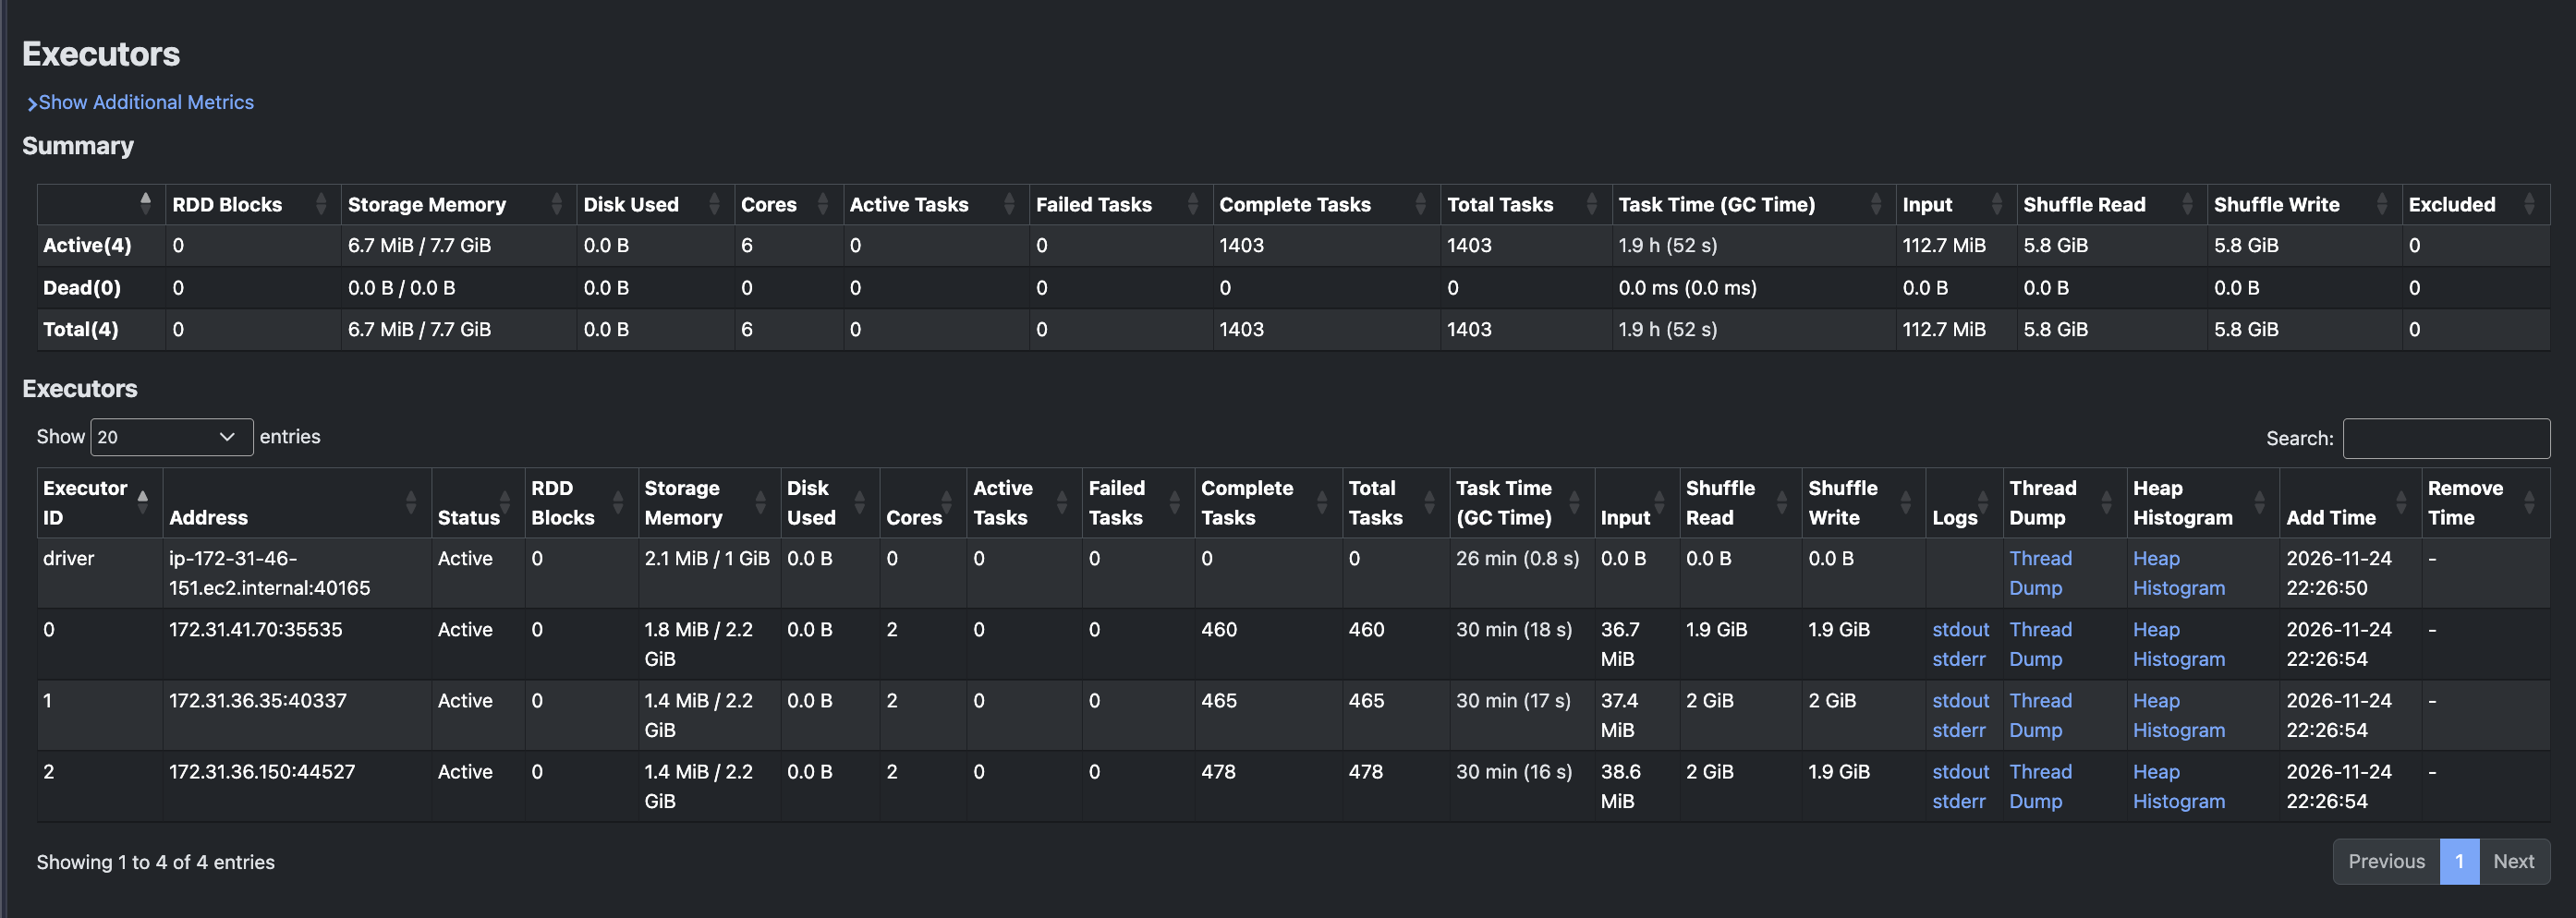
\includegraphics[keepaspectratio]{spark/screenshots/executors.png}}

}

\caption{\label{fig-executors}Saved Spark executor view from the cluster
run.}

\end{figure}%

\subsection{Partitioning and intermediate
tables}\label{partitioning-and-intermediate-tables}

The full stream initially contains 18,250 Parquet files. Repartitioning
by date and rewriting the stream produces 365 files, with an assertion
checking that the 50-million-row count is unchanged. Per-user
\texttt{lag} windows calculate message gaps; session grouping produces
message counts, durations, and city counts. Only small aggregate tables
are collected into pandas for reporting.

\subsection{Reproducibility}\label{reproducibility}

The repository stores simulation settings, notebooks, output CSV files,
and cluster screenshots. This manuscript references those existing
artifacts and has execution disabled, so rendering does not launch
simulation or Spark jobs.

\section{Exploratory Data Analysis}\label{sec-eda}

\subsection{Intent structure and semantic
overlap}\label{intent-structure-and-semantic-overlap}

Part A examines the original 13,083 messages. Assigned risk is
concentrated in account-access and identity intents: 87.5\% of
account-access sentences and 74.5\% of identity sentences are assigned
high risk. These proportions describe the chosen taxonomy, not the
prevalence of fraud in banking conversations.

\begin{figure}

\centering{

\pandocbounded{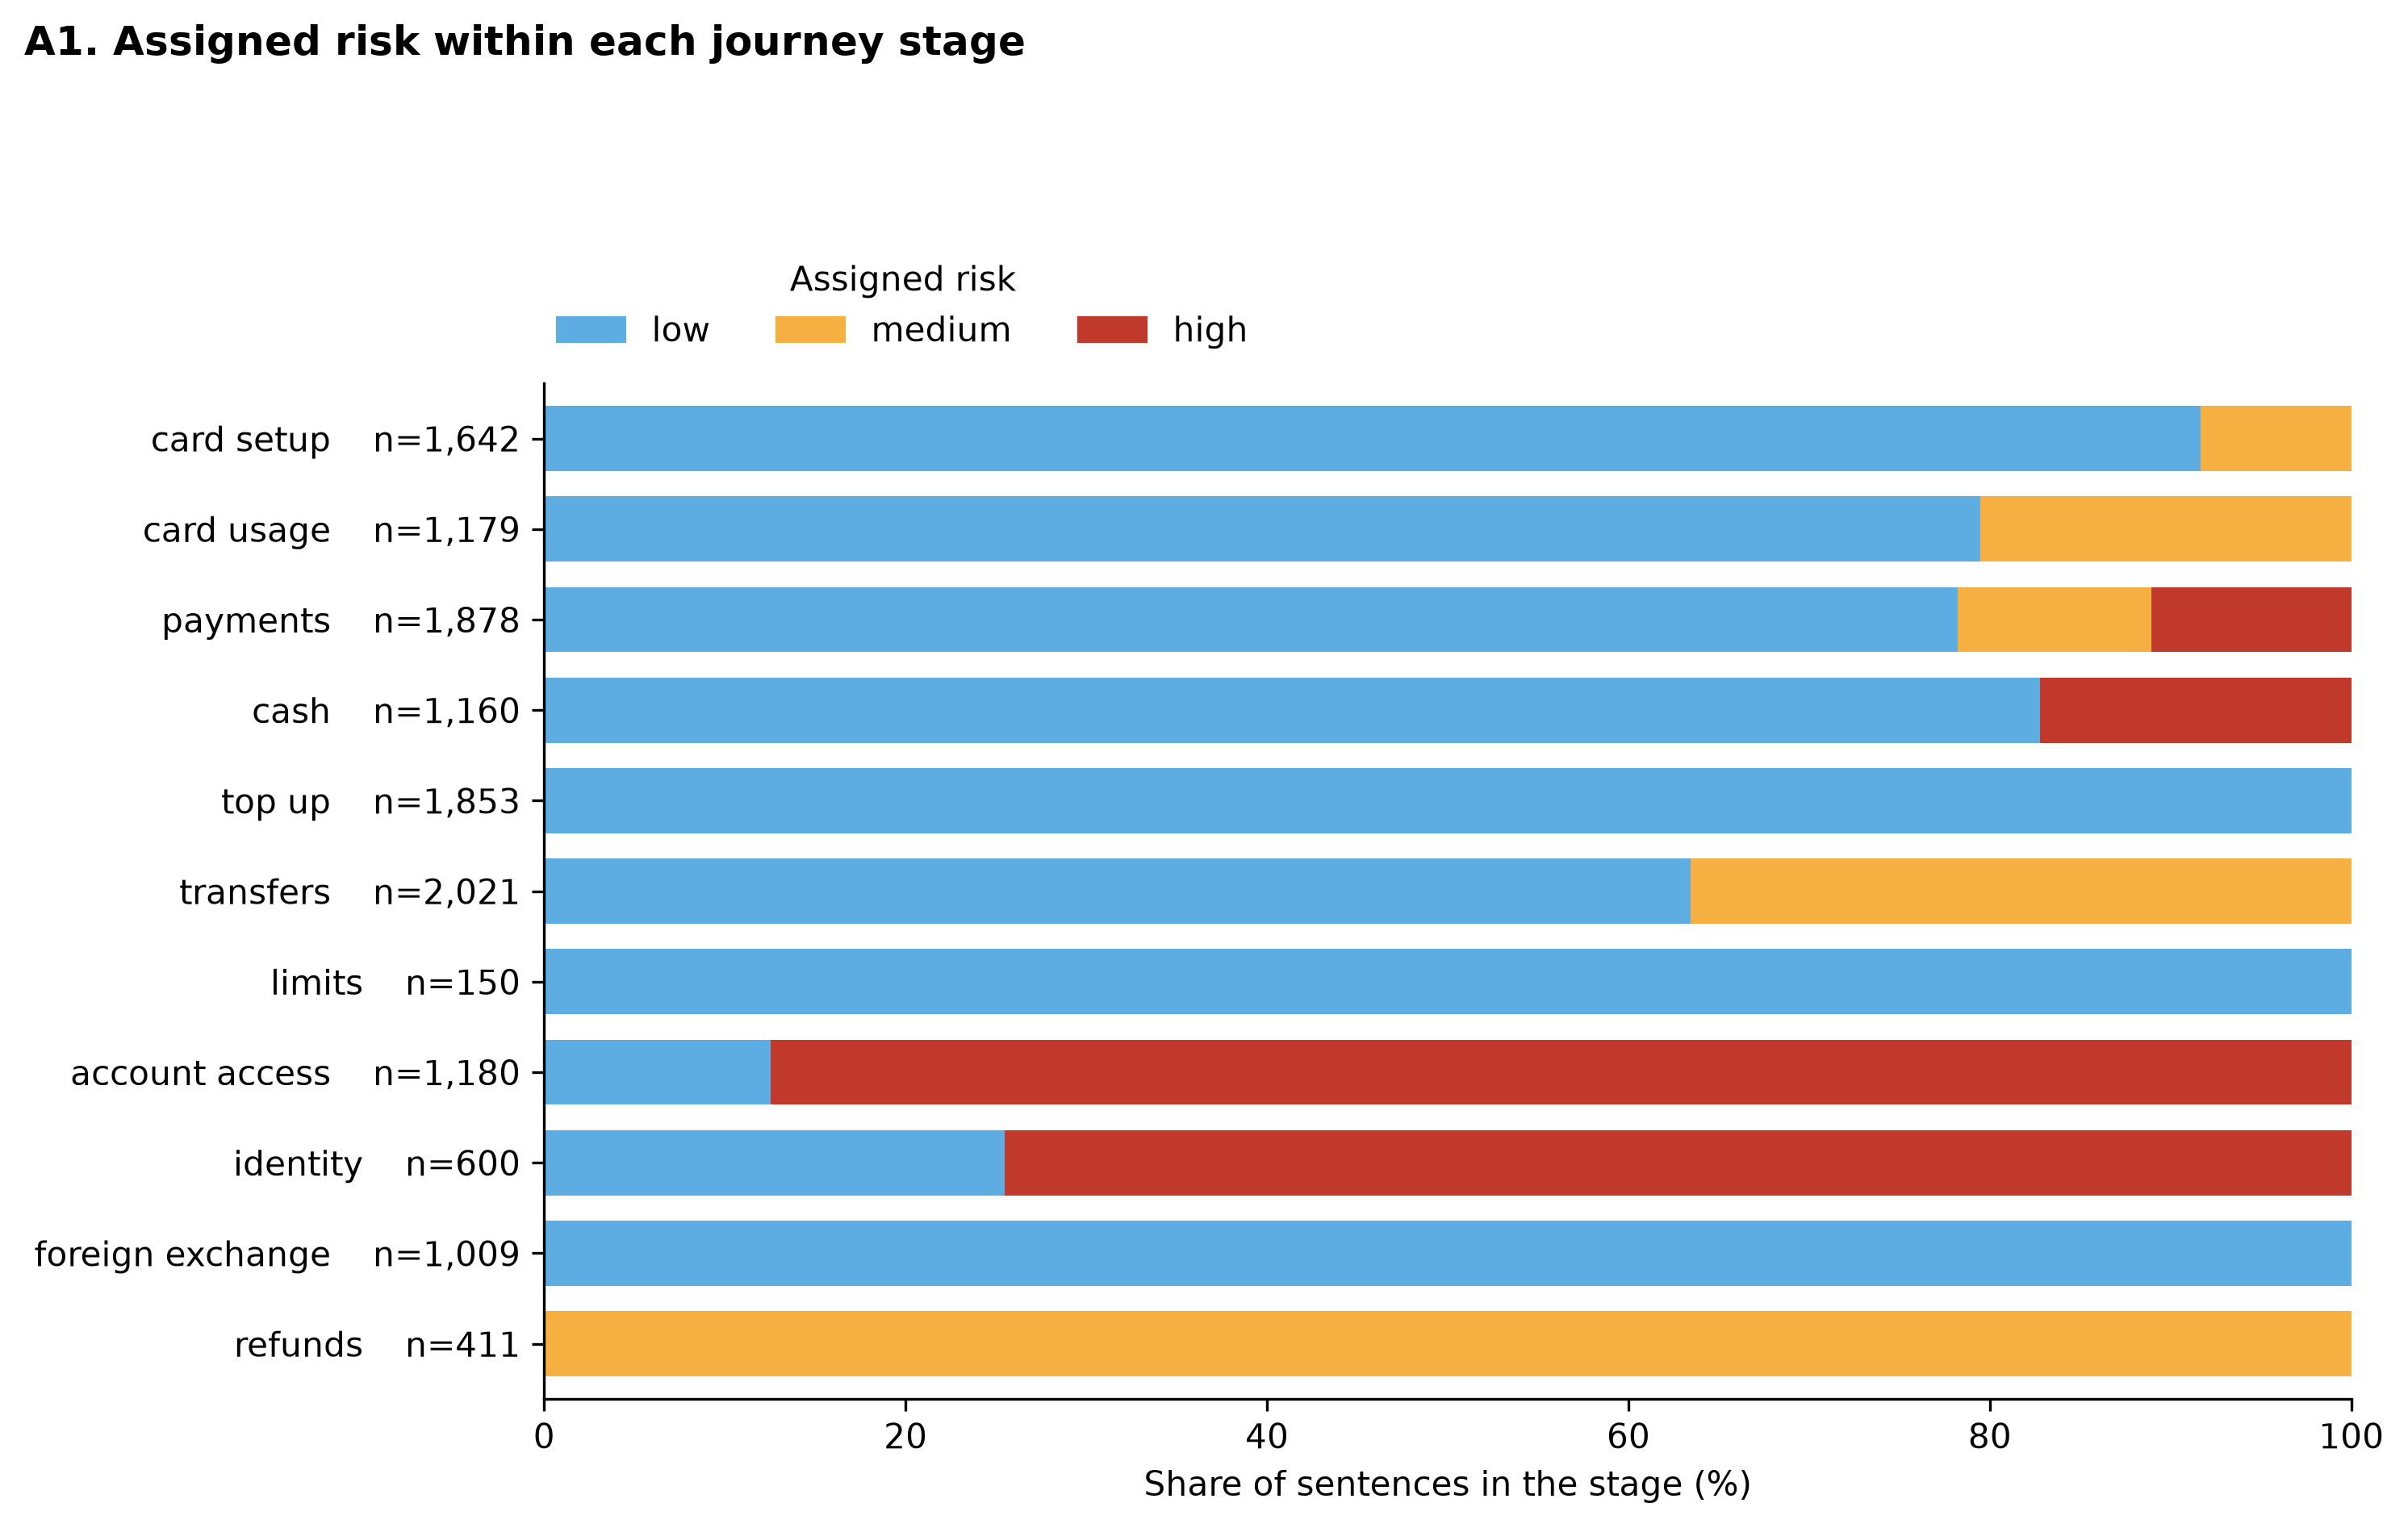
\includegraphics[keepaspectratio]{figures/A_risk_by_stage.png}}

}

\caption{\label{fig-stage-risk}Assigned risk within Banking77 journey
stages.}

\end{figure}%

The semantic map uses MiniLM sentence embeddings and UMAP. The original
embedding space, rather than the two-dimensional plot, supplies the
nearest-neighbor measurements. Identity-related wording remains cohesive
across different intents, whereas apparent account-takeover cohesion is
driven largely by neighbors of the same intent. This cautions against
interpreting visual separation as a detector.

\begin{figure}

\centering{

\pandocbounded{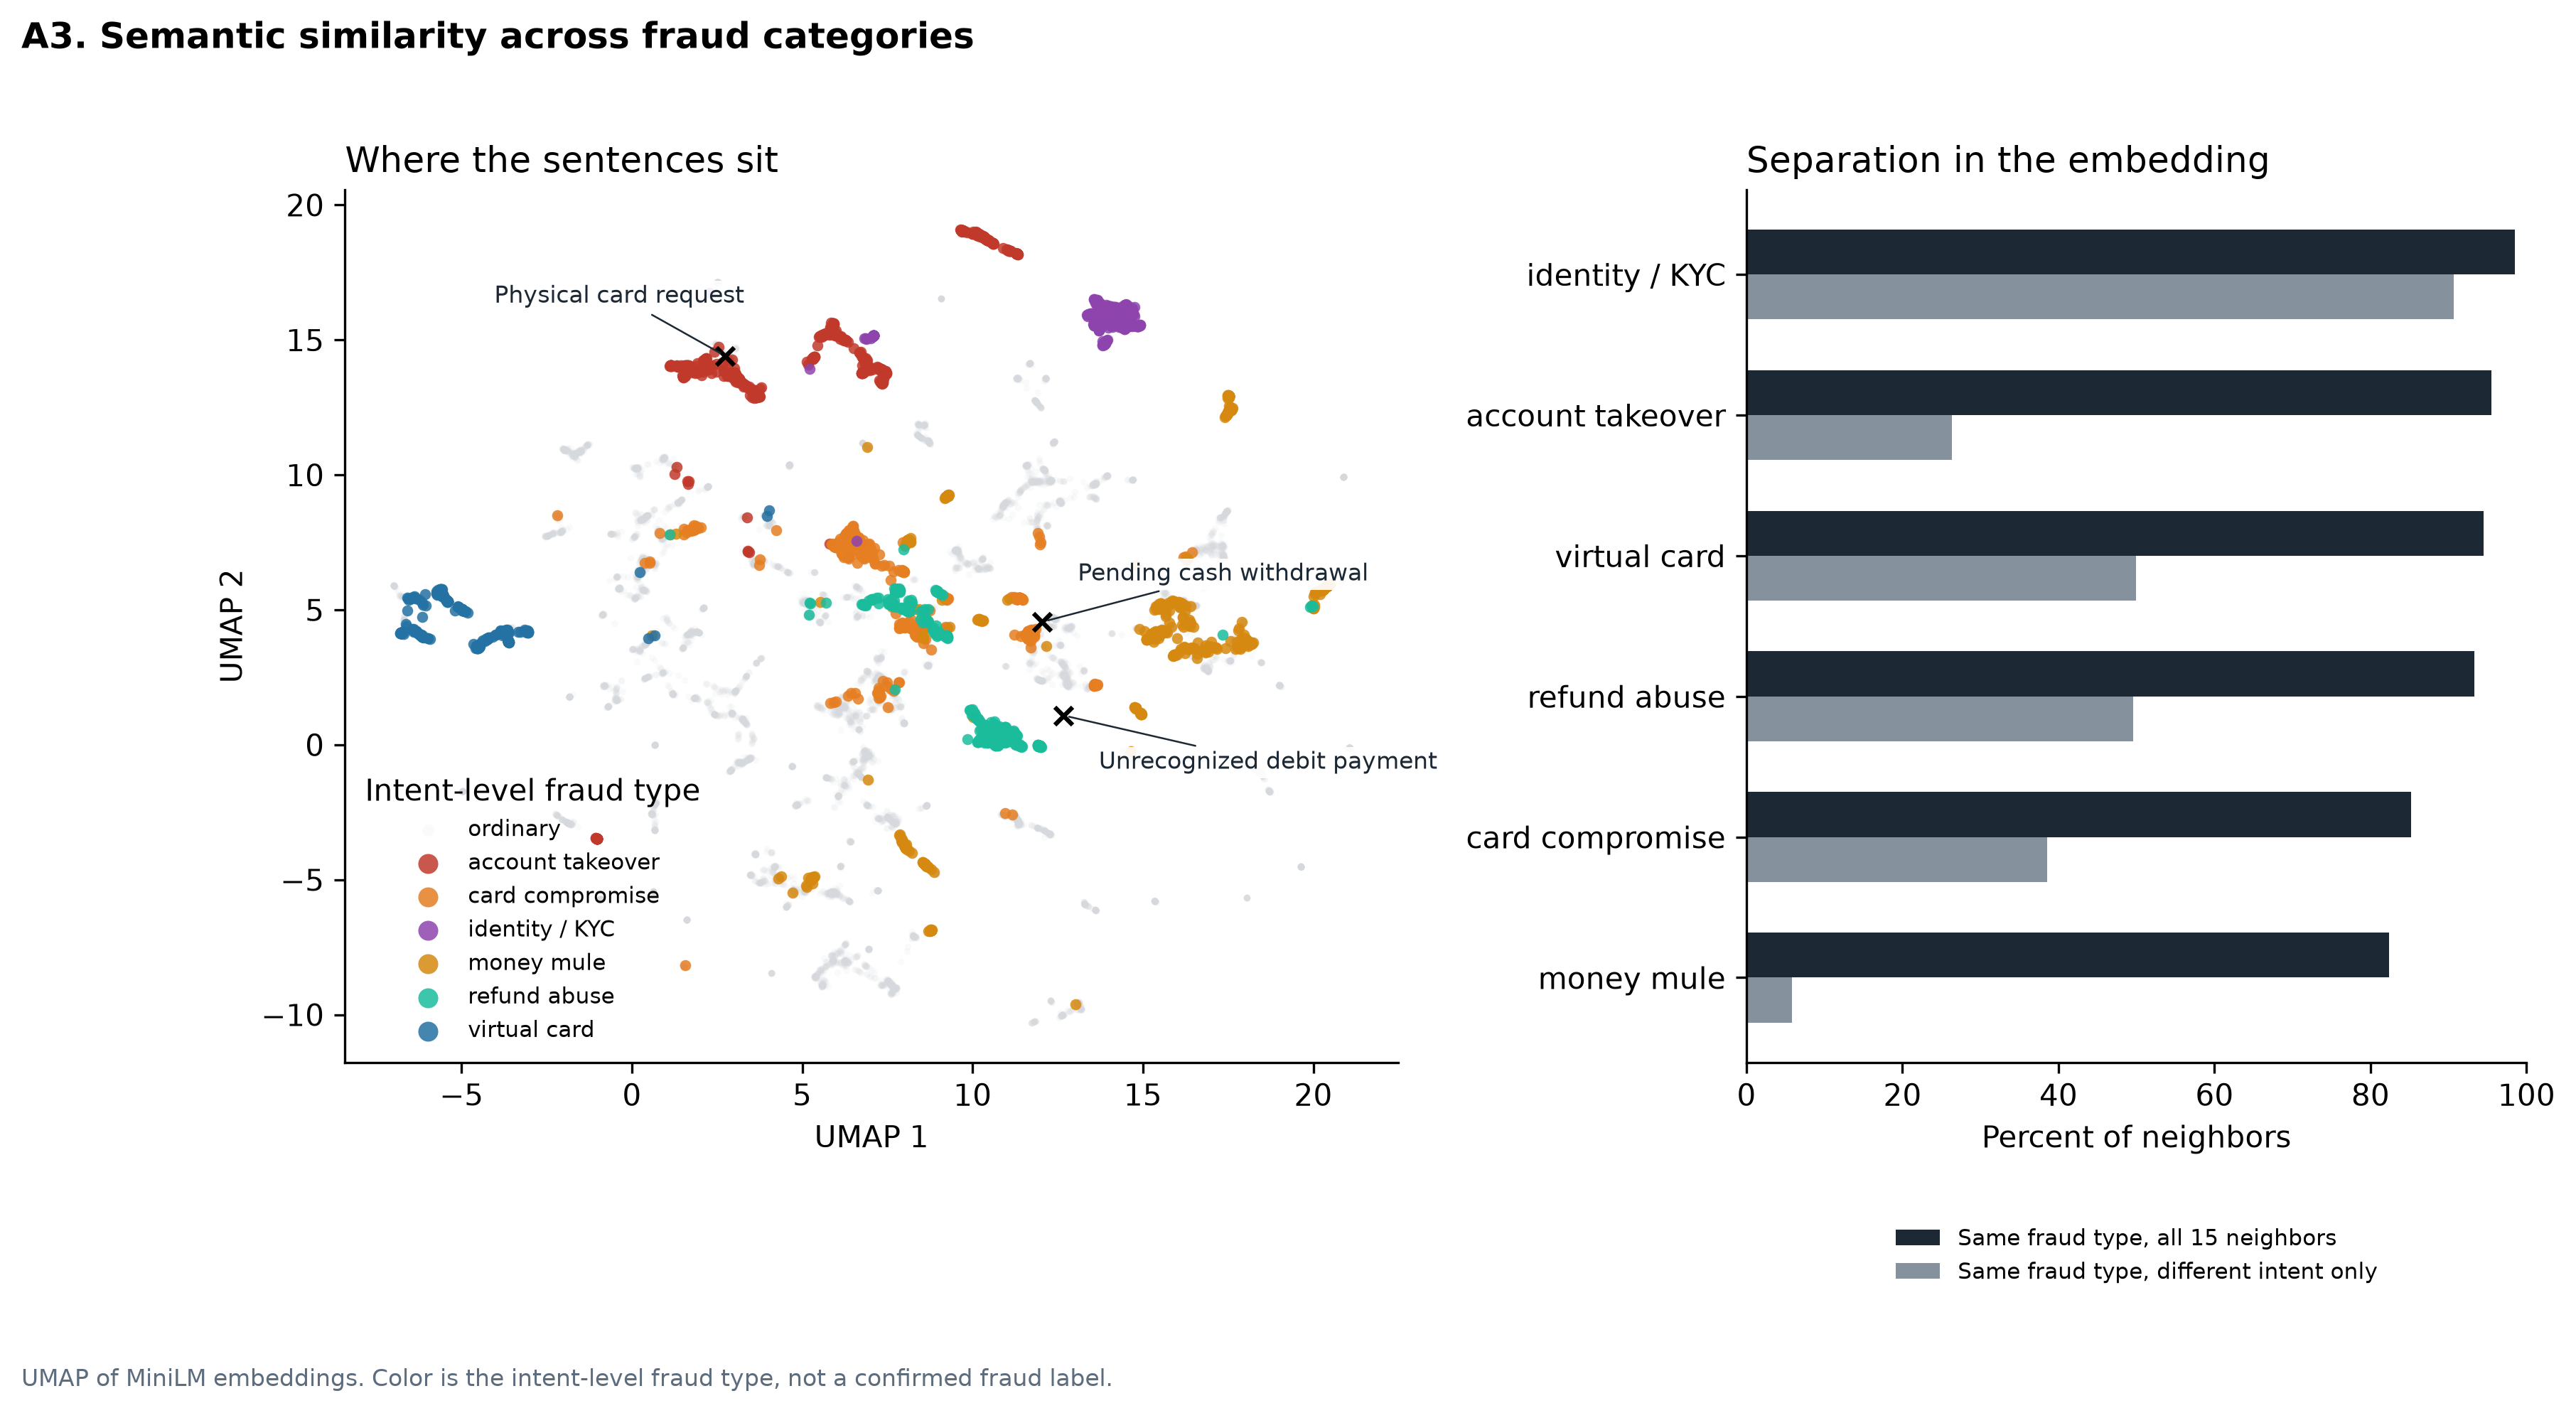
\includegraphics[keepaspectratio]{figures/A_umap.png}}

}

\caption{\label{fig-semantic-map}Semantic map of Banking77 messages,
using sentence embeddings and UMAP.}

\end{figure}%

Median message lengths are 46 characters for low risk, 50 for medium
risk, and 45 for high risk. Length alone provides little descriptive
separation.

\subsection{Text features and intent
confusion}\label{text-features-and-intent-confusion}

Part B fits a TF-IDF/logistic-regression intent baseline and examines
its errors. Its held-out accuracy is 89.06\%. Among 880 test messages
assigned fraud-relevant intents, the analysis reports 56 routed to
ordinary servicing categories. This is taxonomy-based routing error, not
a count of confirmed fraud cases missed.

\begin{figure}

\centering{

\pandocbounded{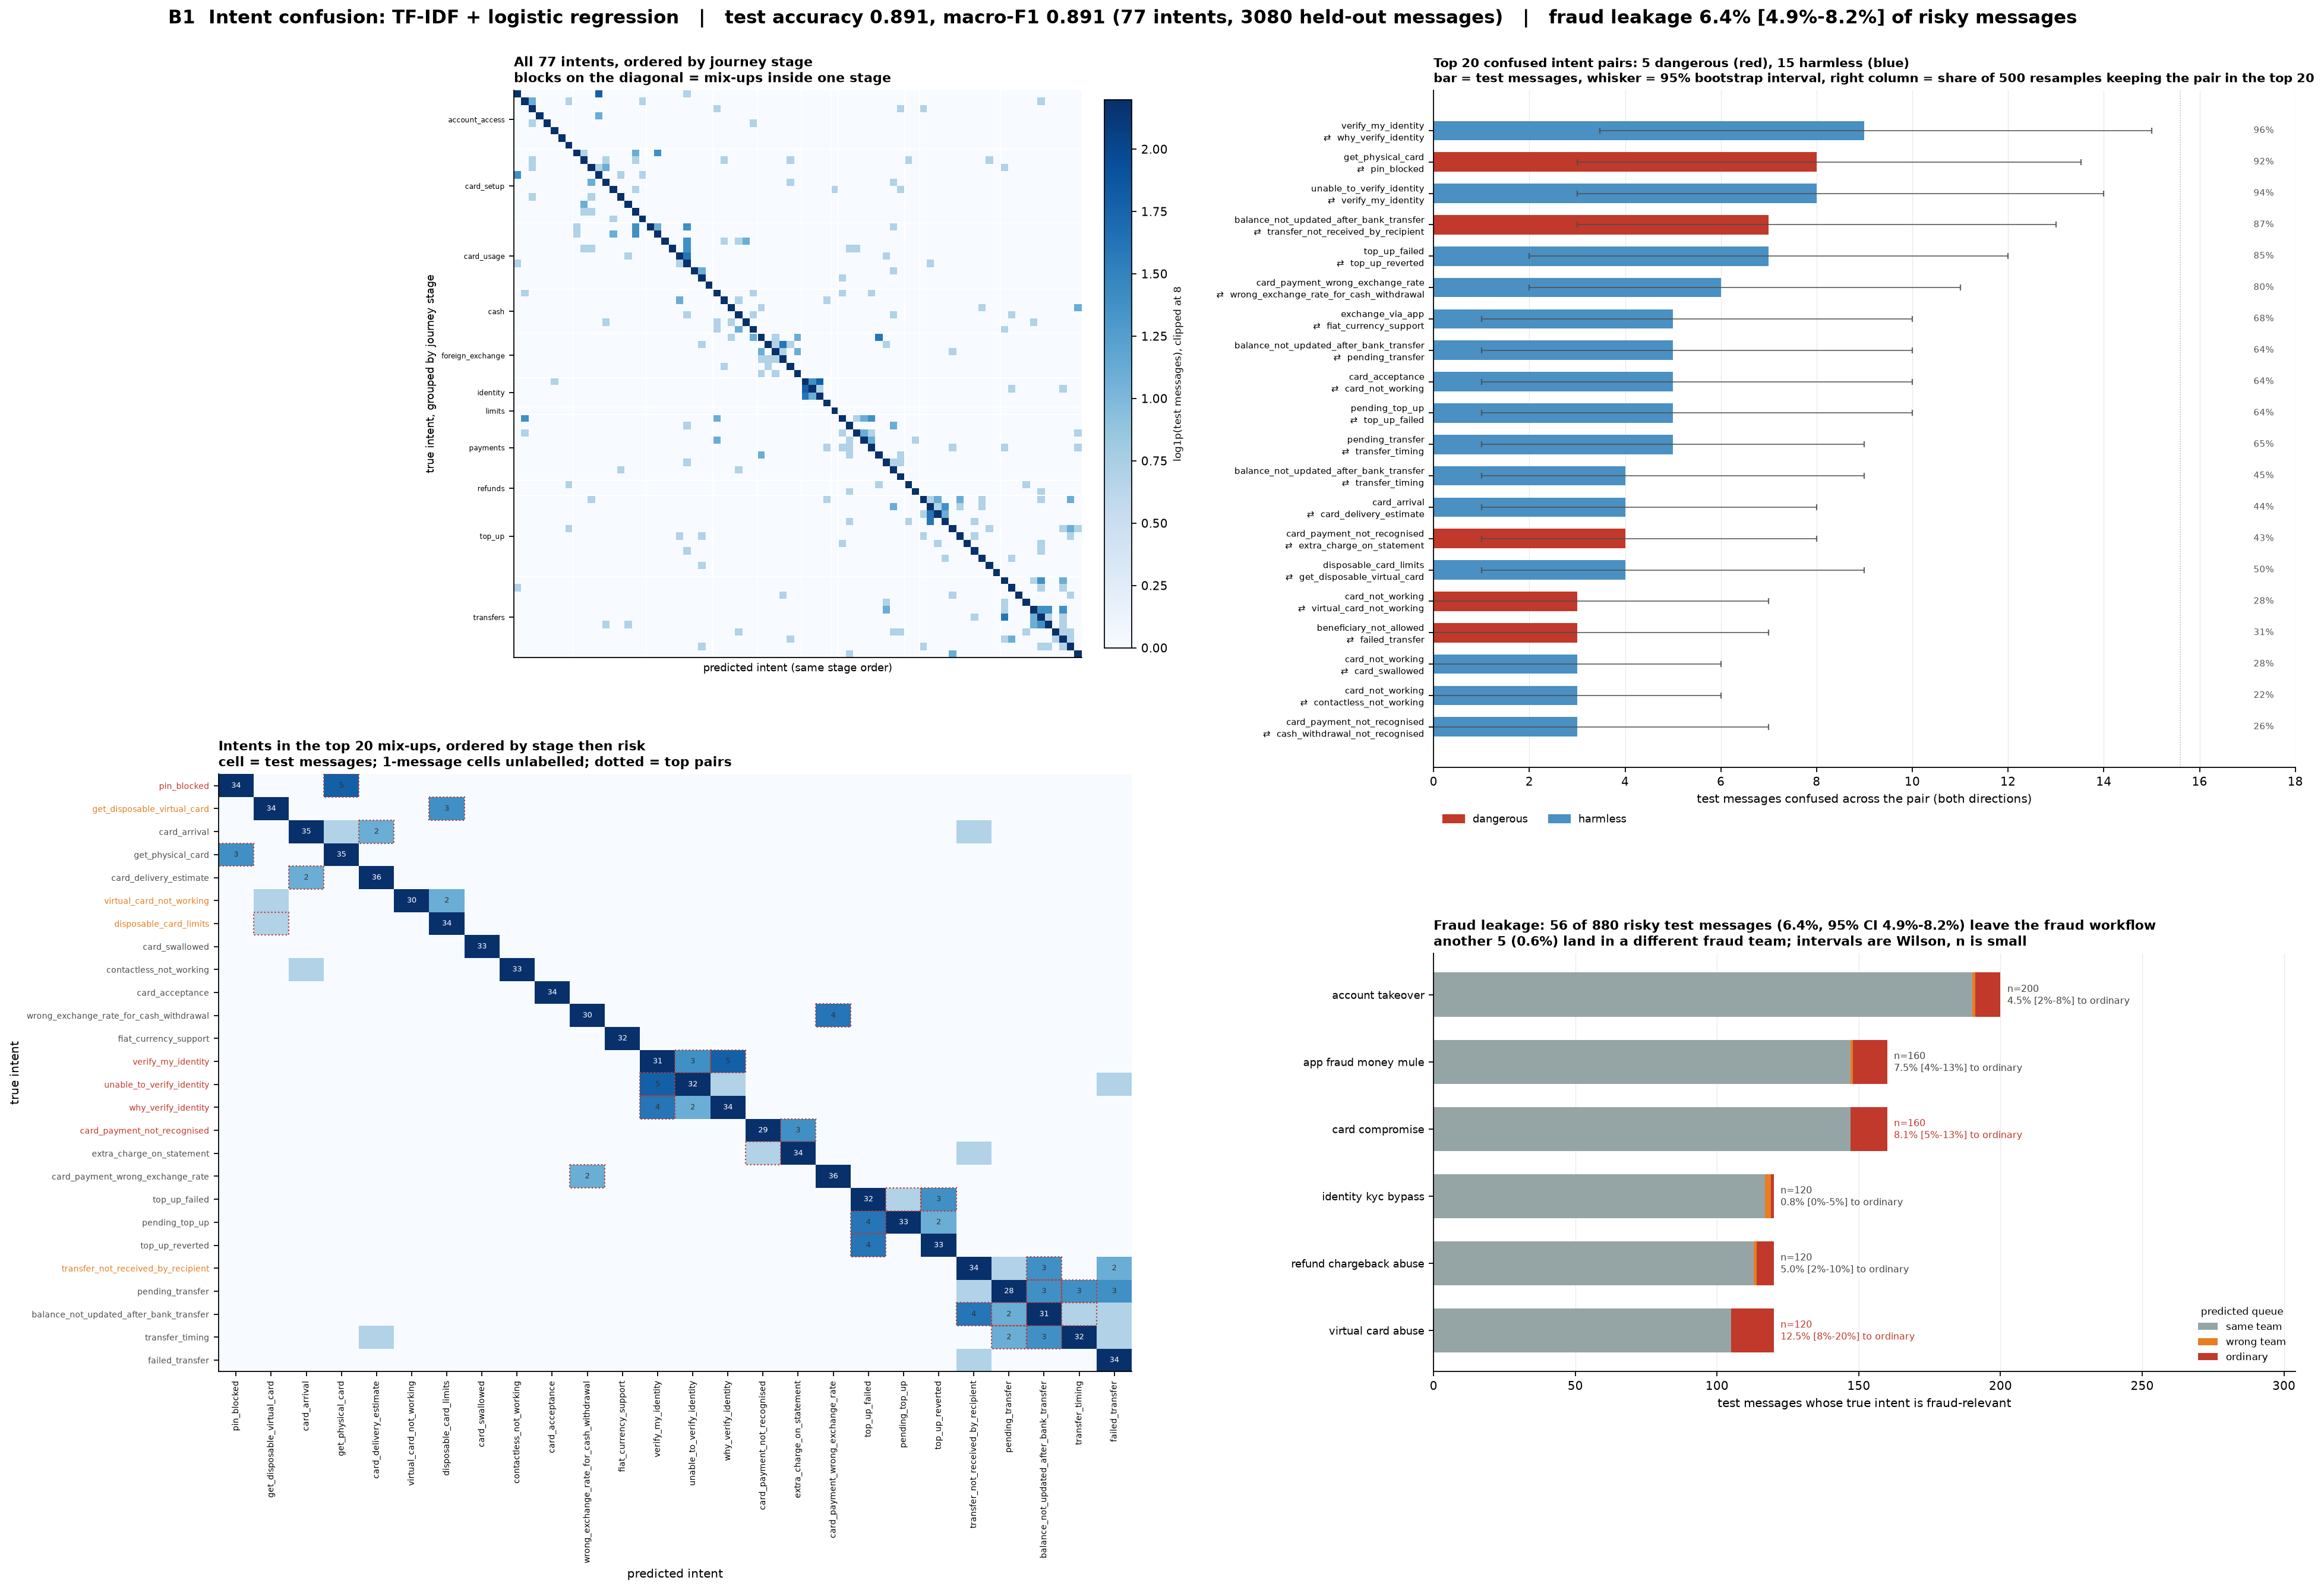
\includegraphics[keepaspectratio]{figures/B_confusion_heatmap.png}}

}

\caption{\label{fig-confusion}Intent confusion and taxonomy-based
routing analysis.}

\end{figure}%

A keyword rule constructed from training text retrieves 678 of 880
fraud-relevant test messages: 77.05\% recall with 28.79\% precision. It
flags 2,355 messages in total, illustrating the false-alert burden of
treating characteristic words as standalone detection rules. Urgency
analysis also finds that incident words such as references to theft are
more informative for some taxonomy groups than generic time-pressure
language.

\begin{figure}

\centering{

\pandocbounded{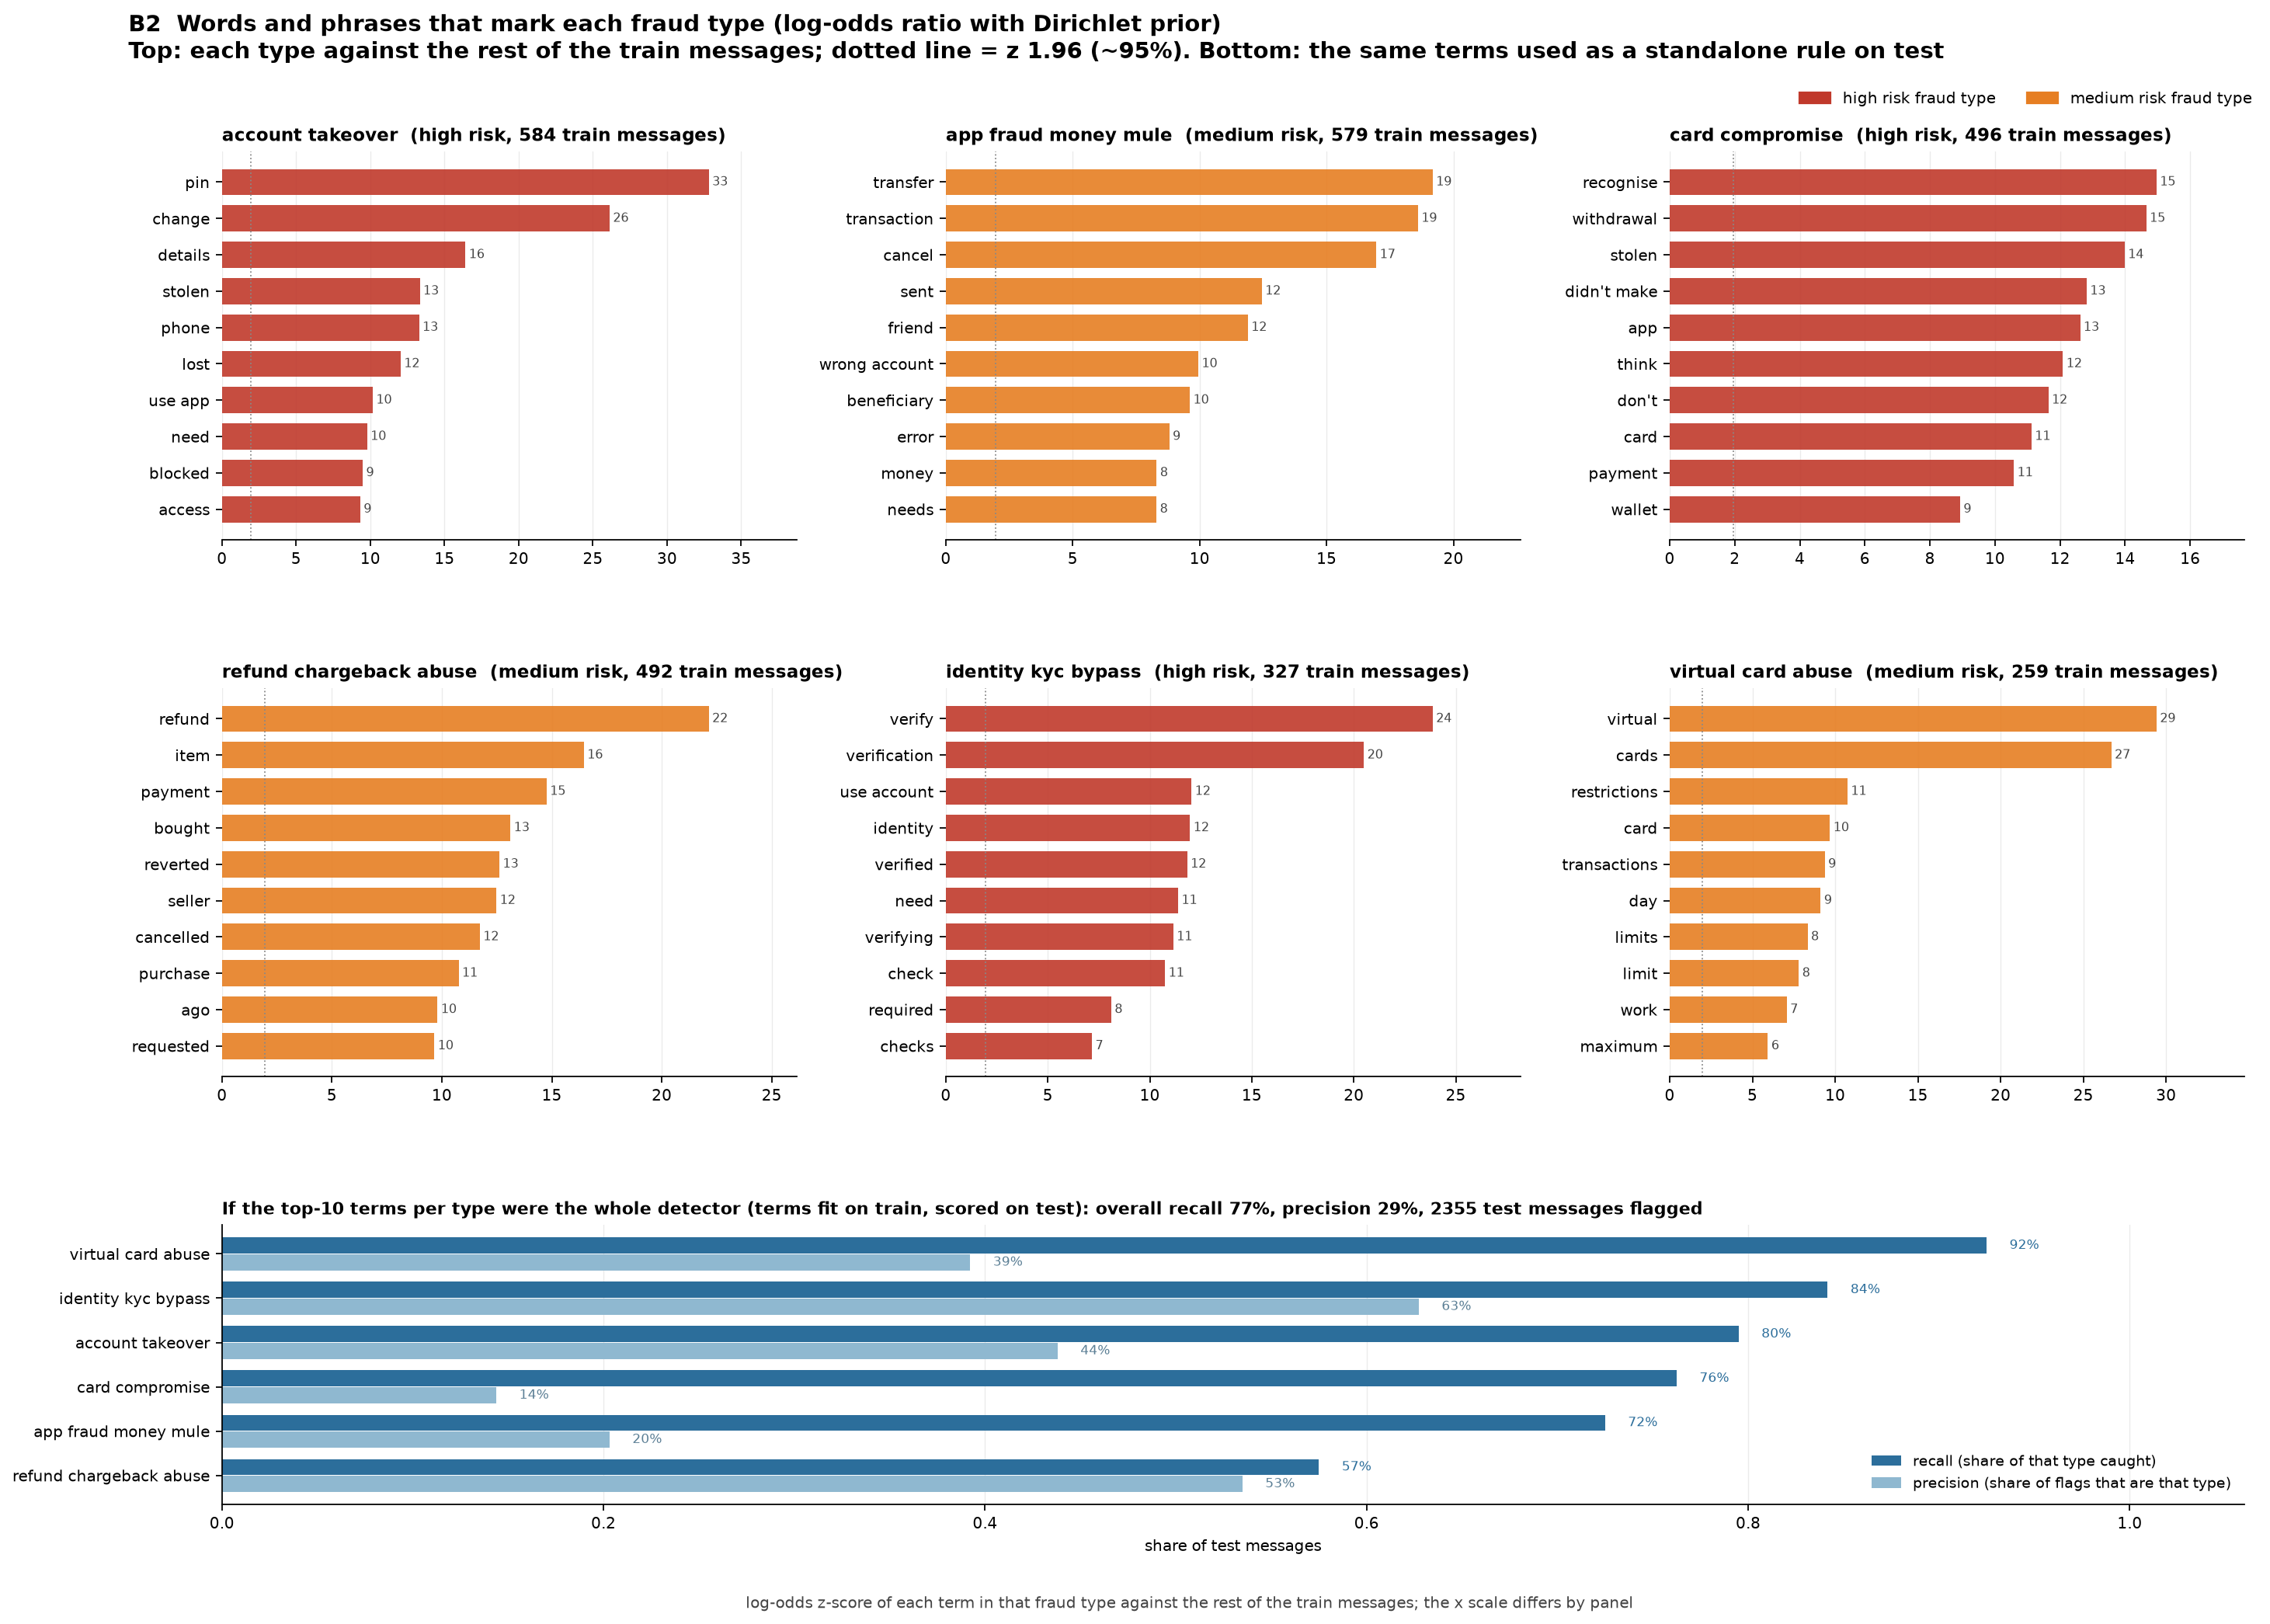
\includegraphics[keepaspectratio]{figures/B_keywords_by_fraud_type.png}}

}

\caption{\label{fig-keywords}Characteristic language and held-out
keyword-rule evaluation.}

\end{figure}%

\begin{figure}

\centering{

\pandocbounded{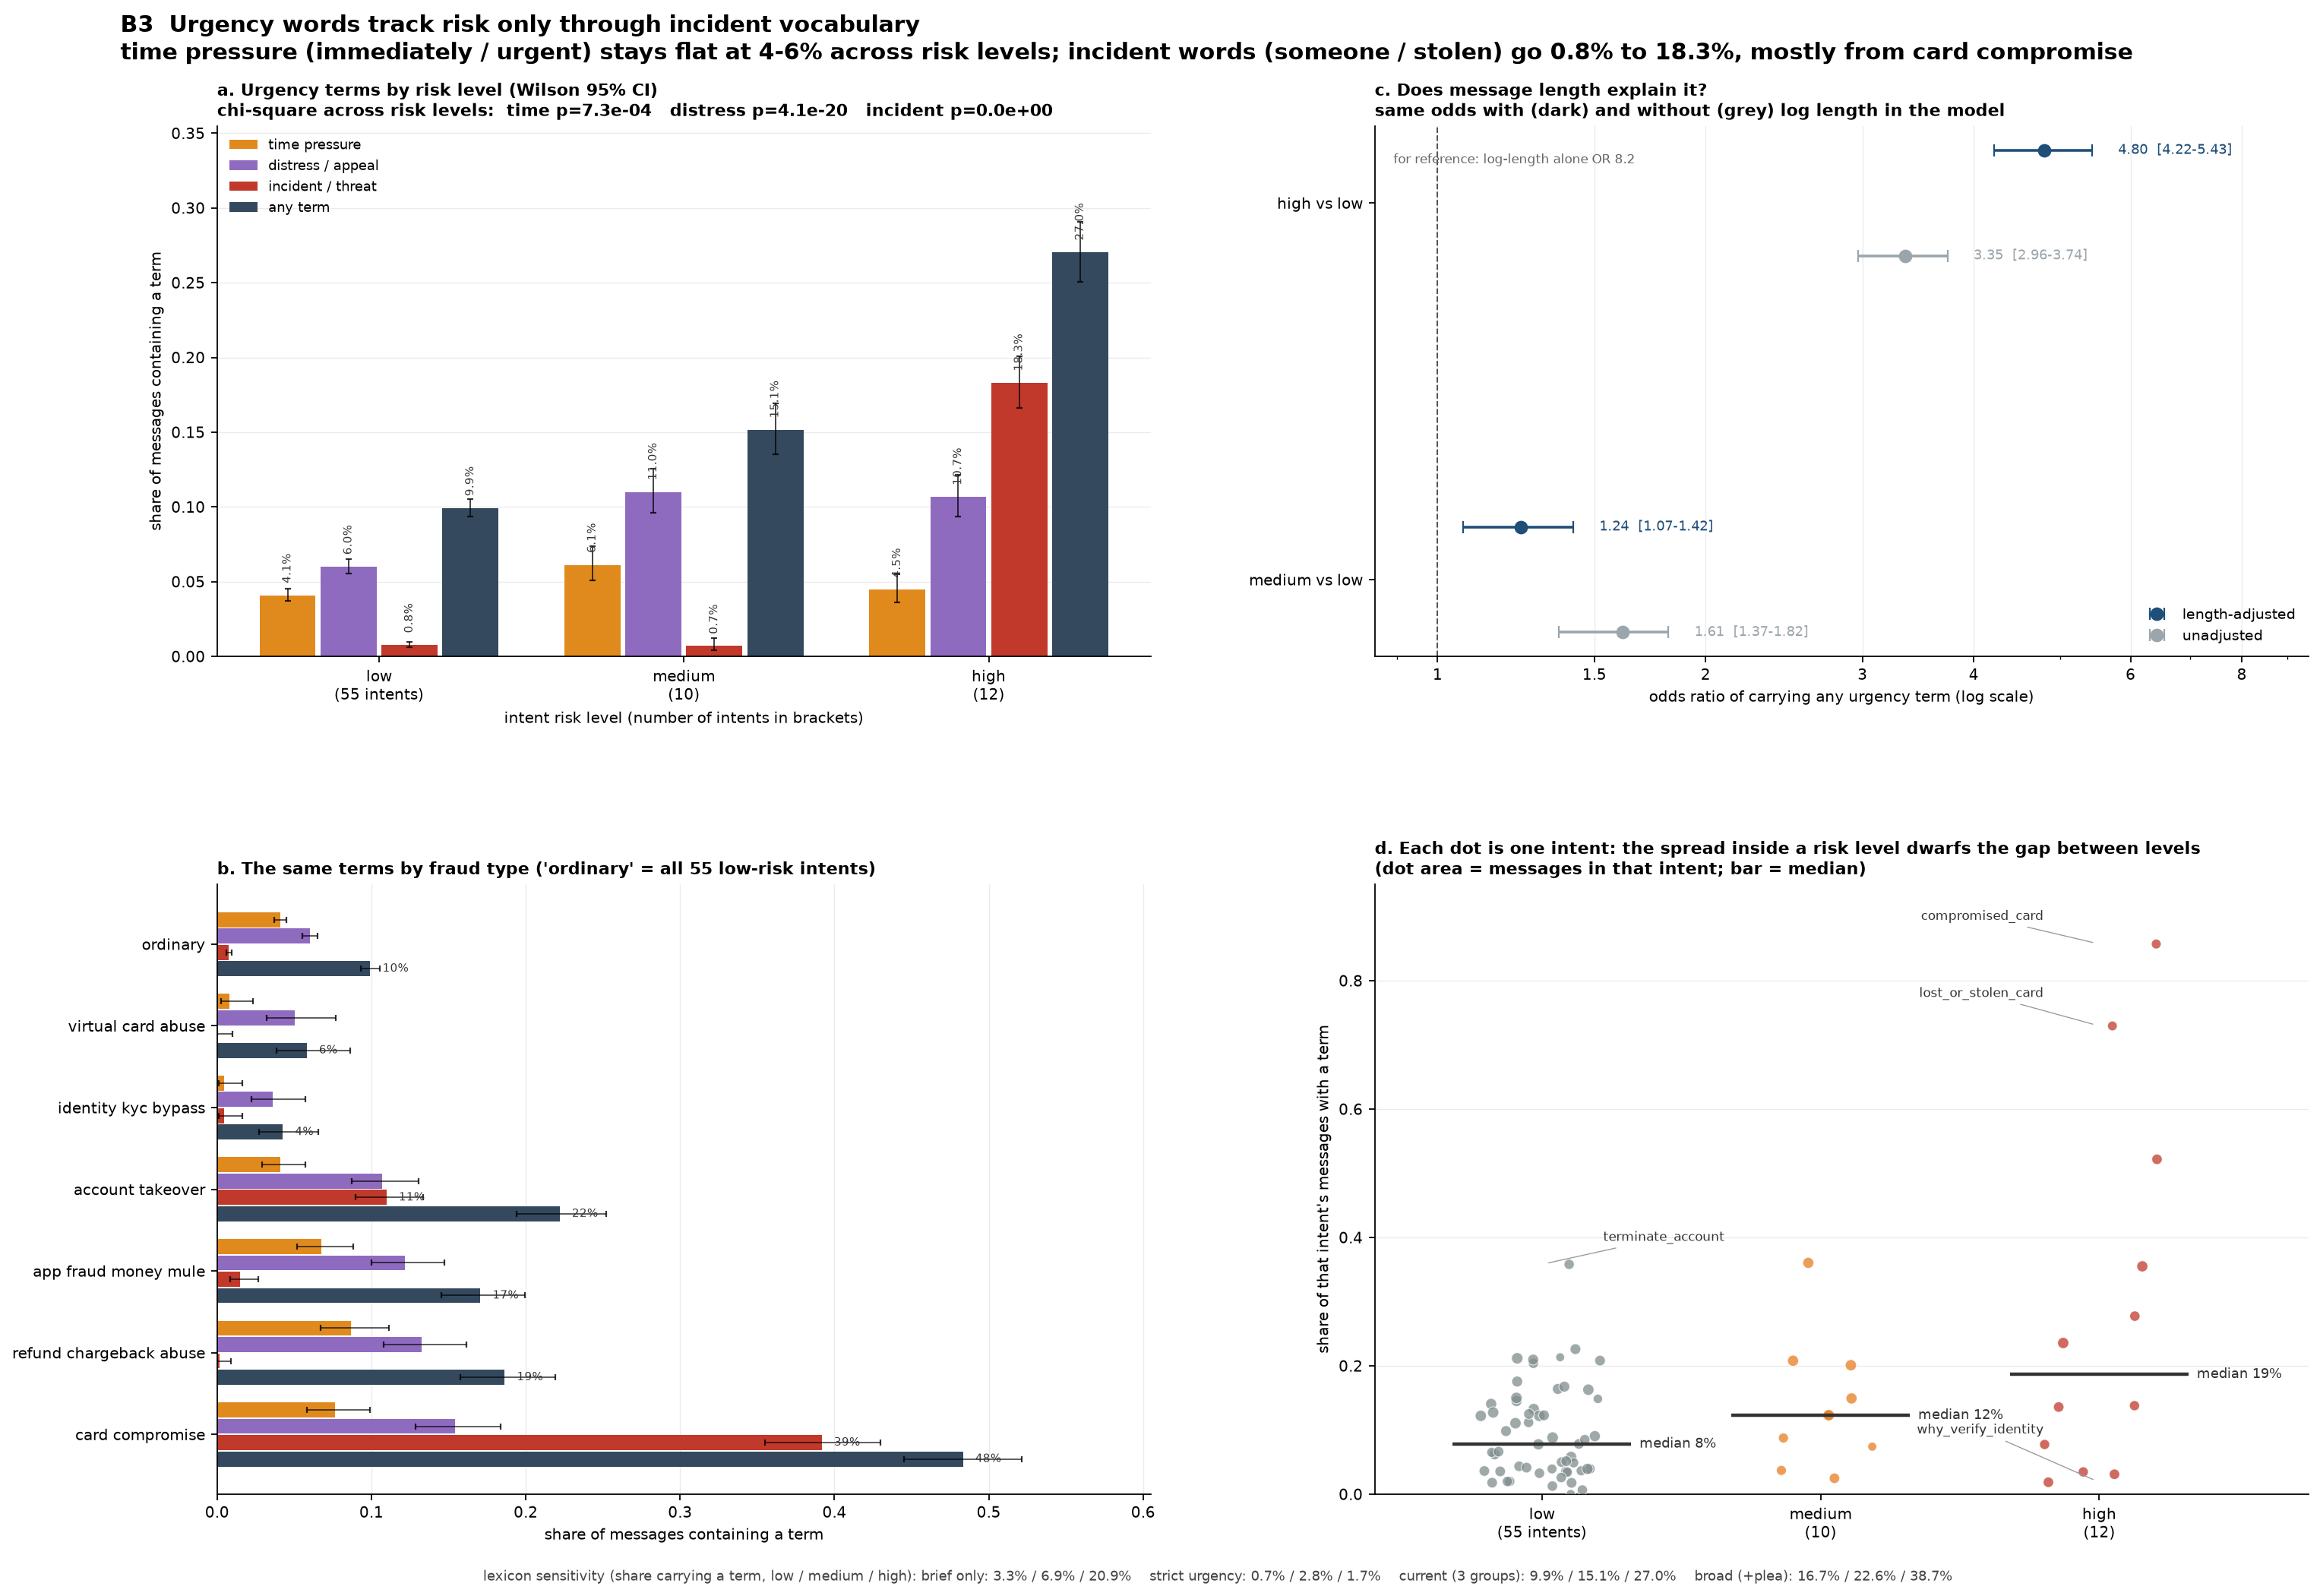
\includegraphics[keepaspectratio]{figures/B_urgency_by_risk.png}}

}

\caption{\label{fig-urgency}Urgency and incident language across
assigned risk groups.}

\end{figure}%

\subsection{Temporal and session
behavior}\label{temporal-and-session-behavior}

Parts C and D visualize the development stream. Their patterns reflect
the simulation rules. Ordinary sessions typically contain three messages
and last six minutes. Development-stream card-testing sessions have a
median of eleven messages over seventeen minutes; money-mule sessions
span much longer intervals. These are descriptive contrasts rather than
measured predictive performance.

\begin{figure}

\centering{

\pandocbounded{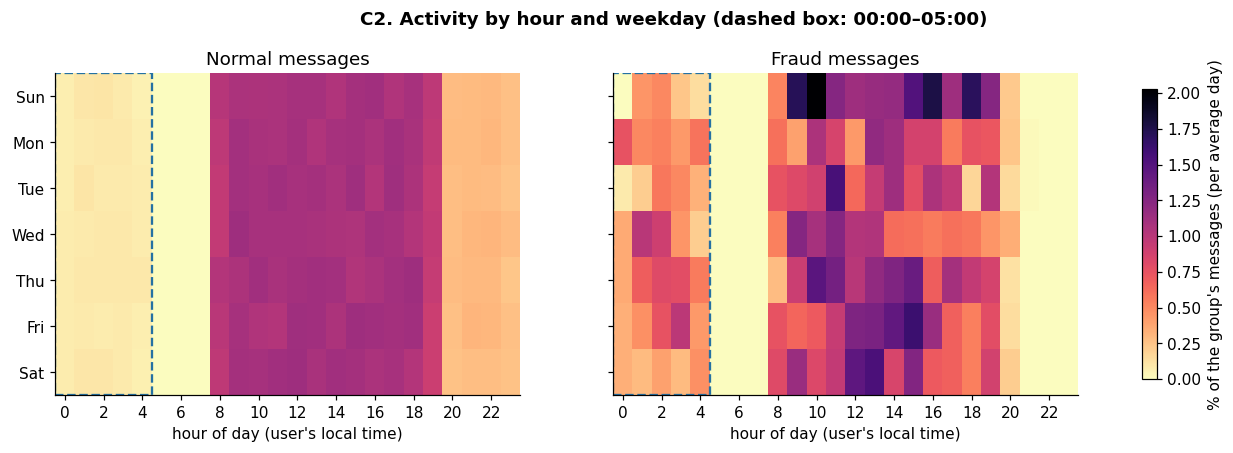
\includegraphics[keepaspectratio]{figures/C2_hour_weekday.png}}

}

\caption{\label{fig-hour-weekday}Development-stream activity by hour and
weekday.}

\end{figure}%

\begin{figure}

\centering{

\pandocbounded{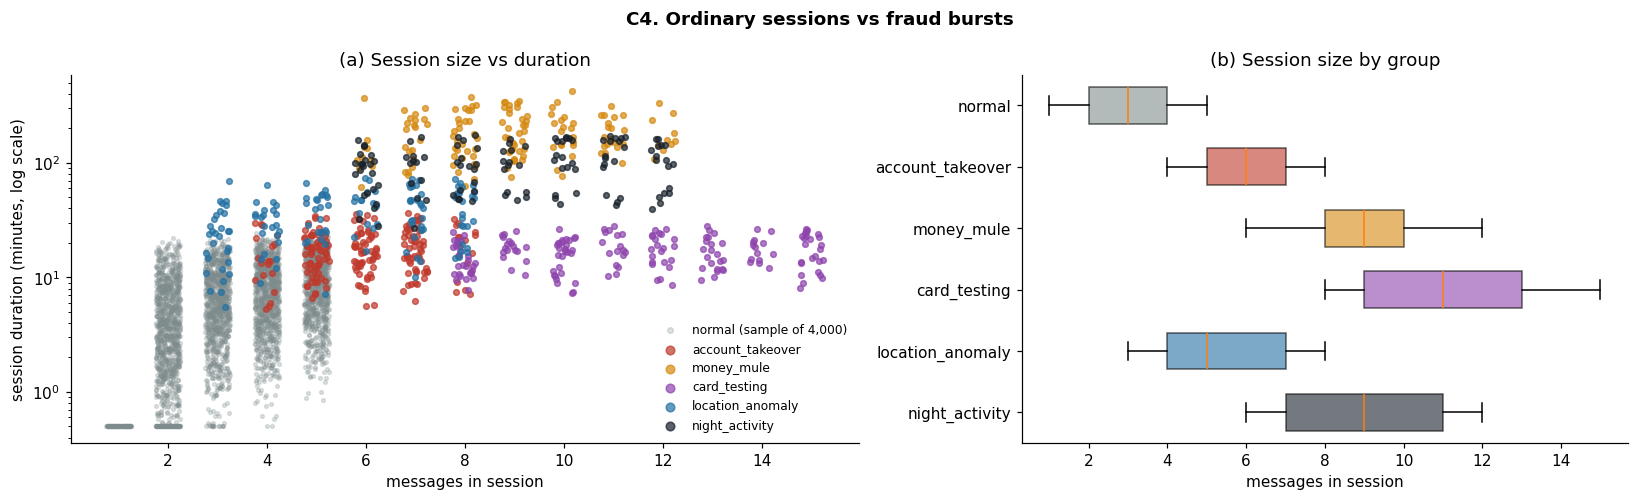
\includegraphics[keepaspectratio]{figures/C4_sessions.png}}

}

\caption{\label{fig-sessions}Development-stream session size and
duration.}

\end{figure}%

The full-stream Spark analysis supports similar descriptive comparisons.
Its median within-session message gap is 115 seconds for ordinary
messages, 64 seconds for card testing, and 143 seconds for account
takeover. Message speed therefore does not isolate every simulated fraud
pattern.

\subsection{Intent sequences and
geography}\label{intent-sequences-and-geography}

Part D examines adjacent intent transitions within sessions, distance
from the user's simulated home city, and intent co-occurrence.
Account-takeover sequences move from account-access topics toward
transfers by construction. Location-anomaly bursts occur away from home,
but ordinary trips also occur away from home, so distance alone is not
equivalent to fraud.

For descriptive sequence analysis, missing intent labels are recovered
through text lookup against the source catalog after consistency checks.
This is not a demonstration of model accuracy on unseen wording.

\begin{figure}

\centering{

\pandocbounded{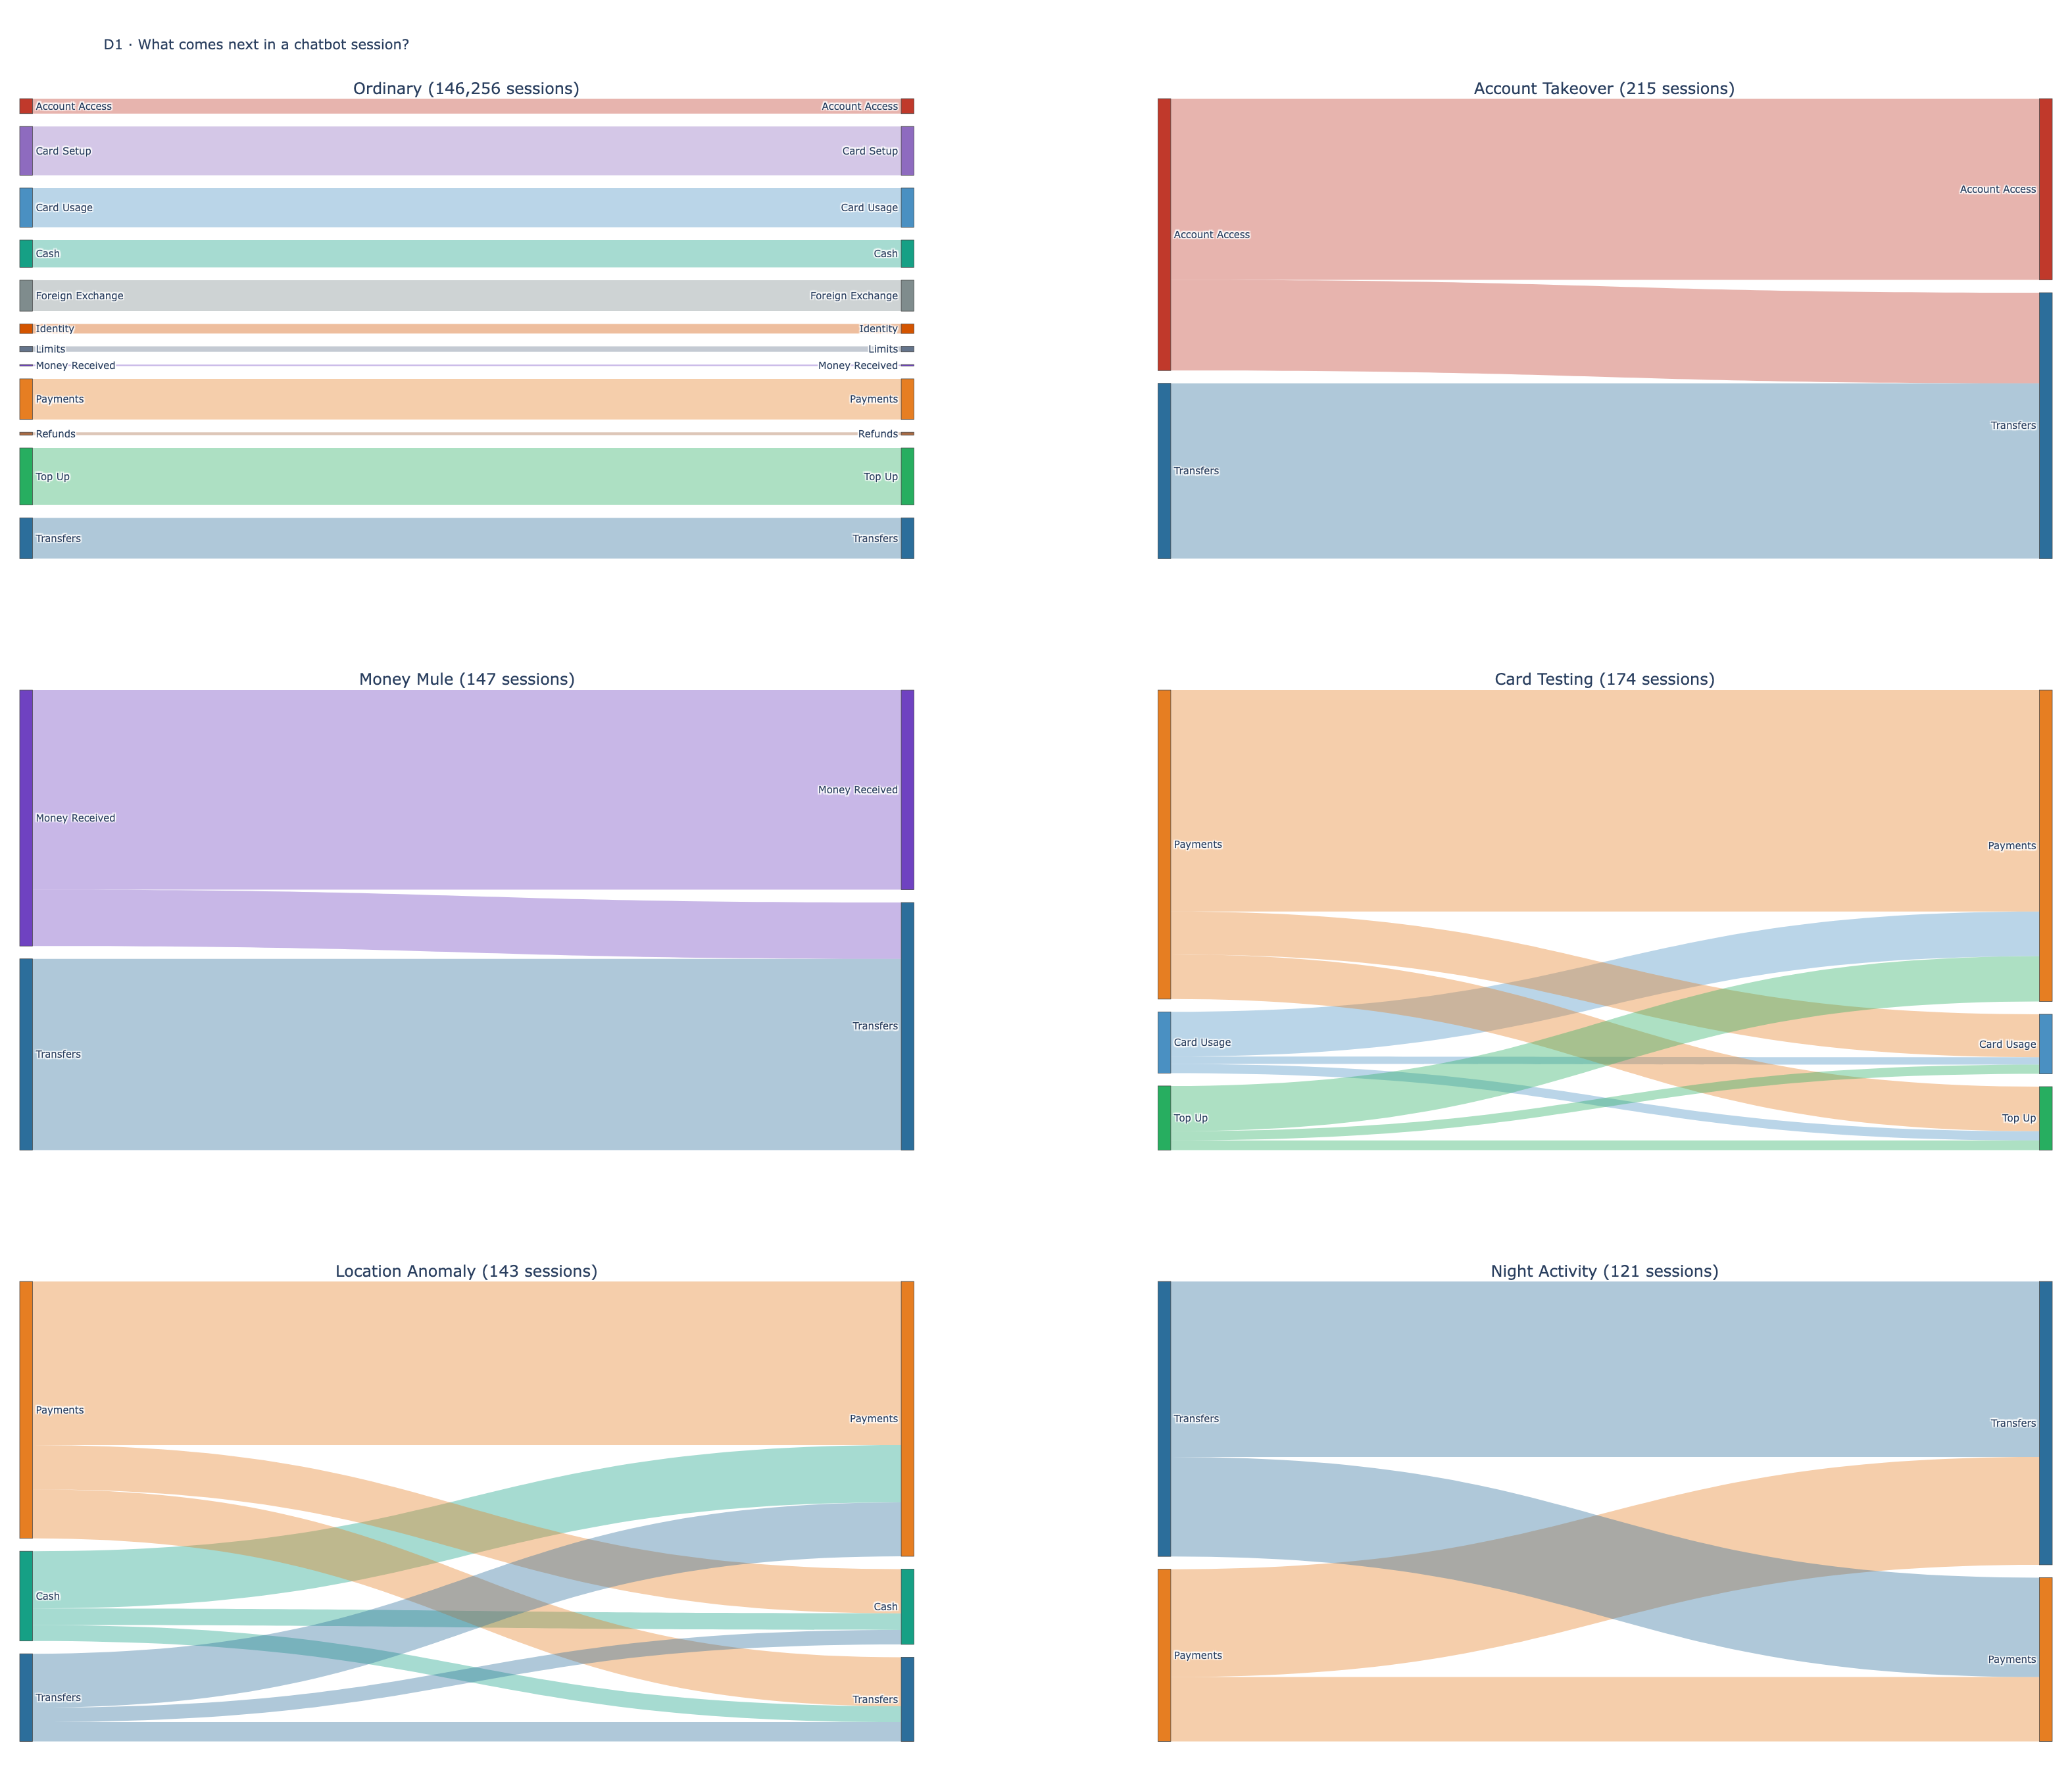
\includegraphics[keepaspectratio]{figures/D1_intent_sequence_sankey.png}}

}

\caption{\label{fig-sequences}Adjacent topic transitions within
development-stream sessions.}

\end{figure}%

\begin{figure}

\centering{

\pandocbounded{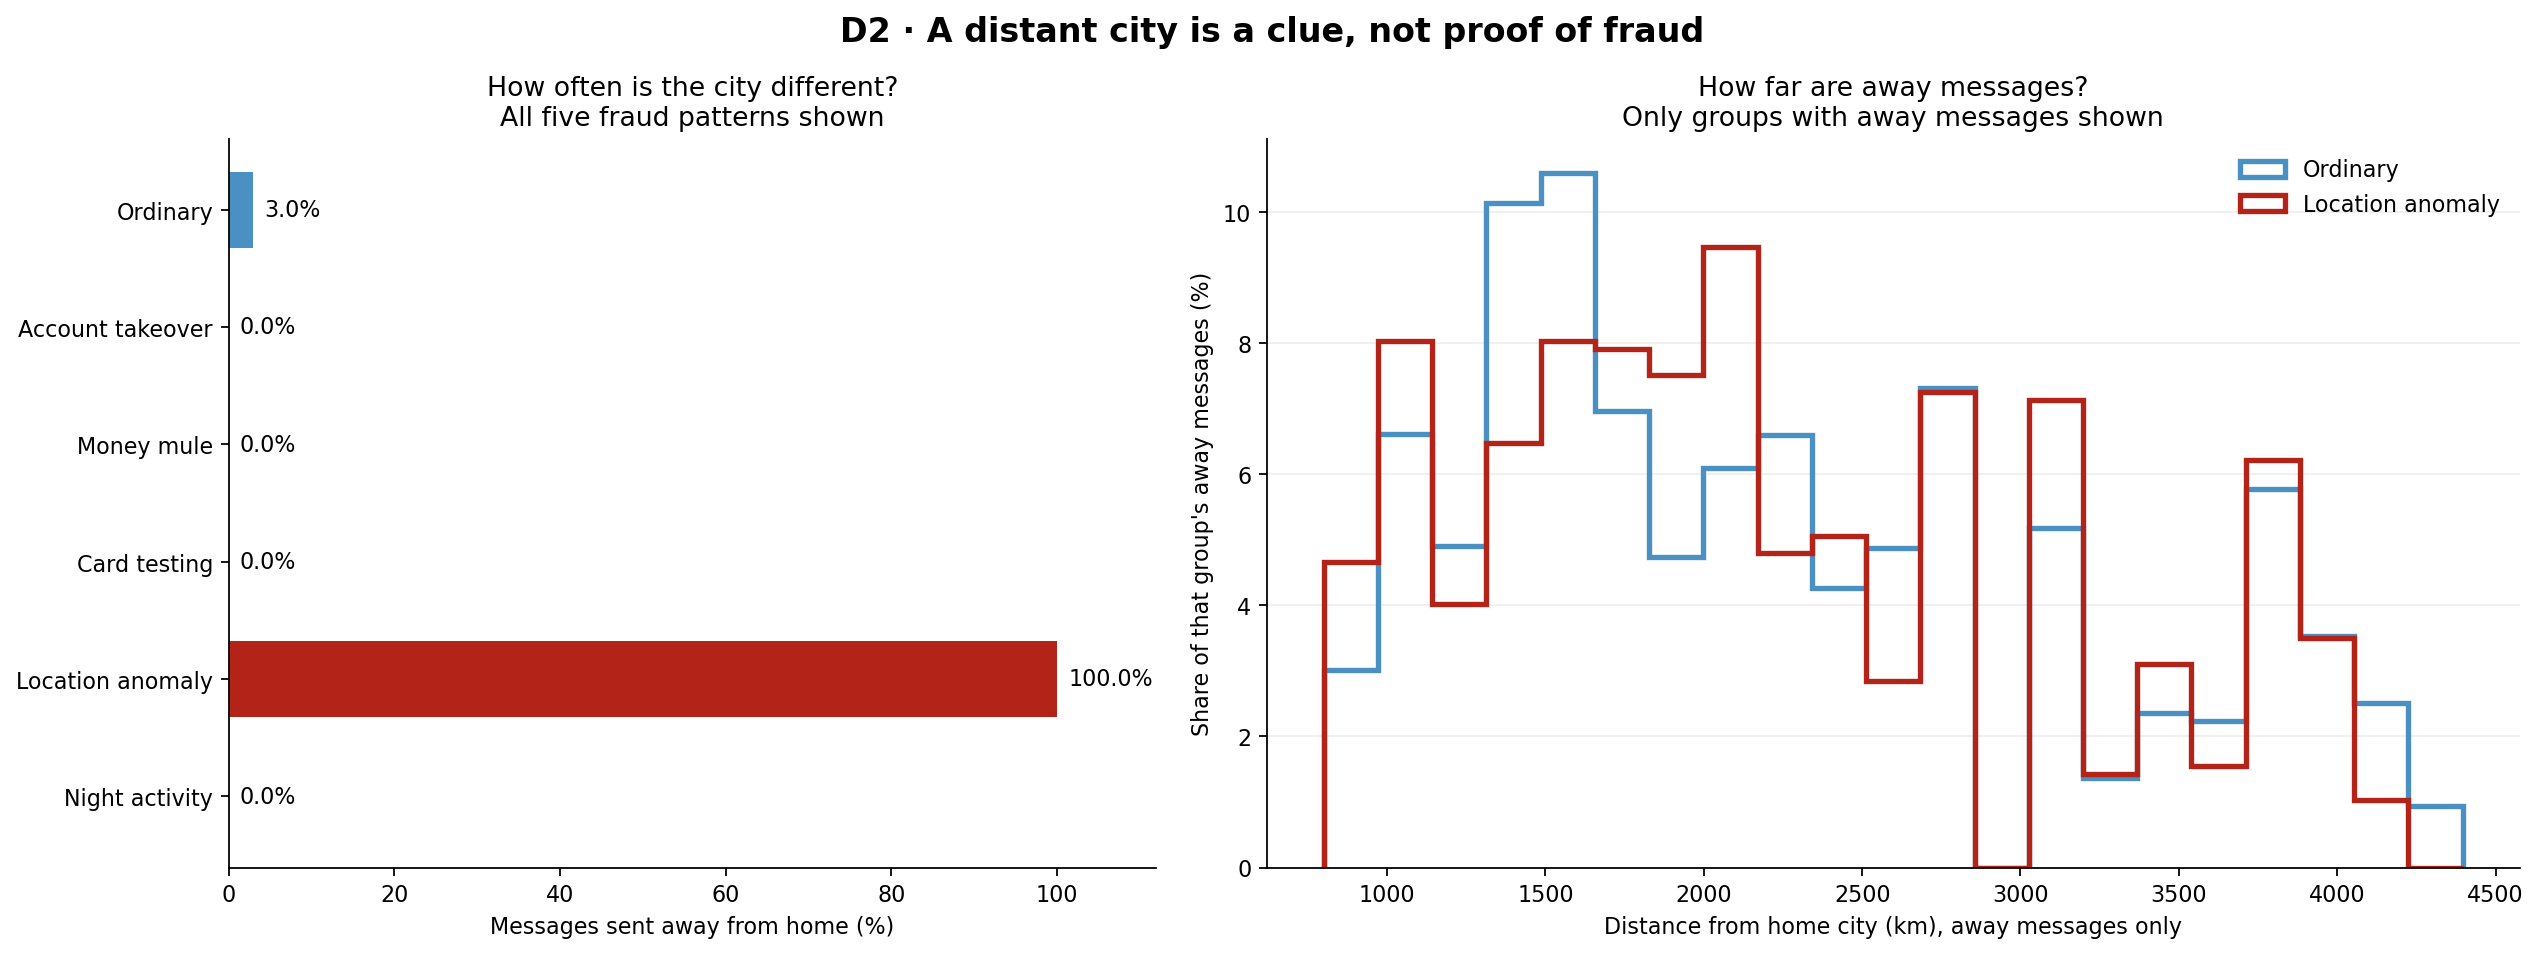
\includegraphics[keepaspectratio]{figures/D2_distance_from_home.png}}

}

\caption{\label{fig-distance}Distance from simulated home city,
comparing ordinary messages and fraud patterns.}

\end{figure}%

\begin{figure}

\centering{

\pandocbounded{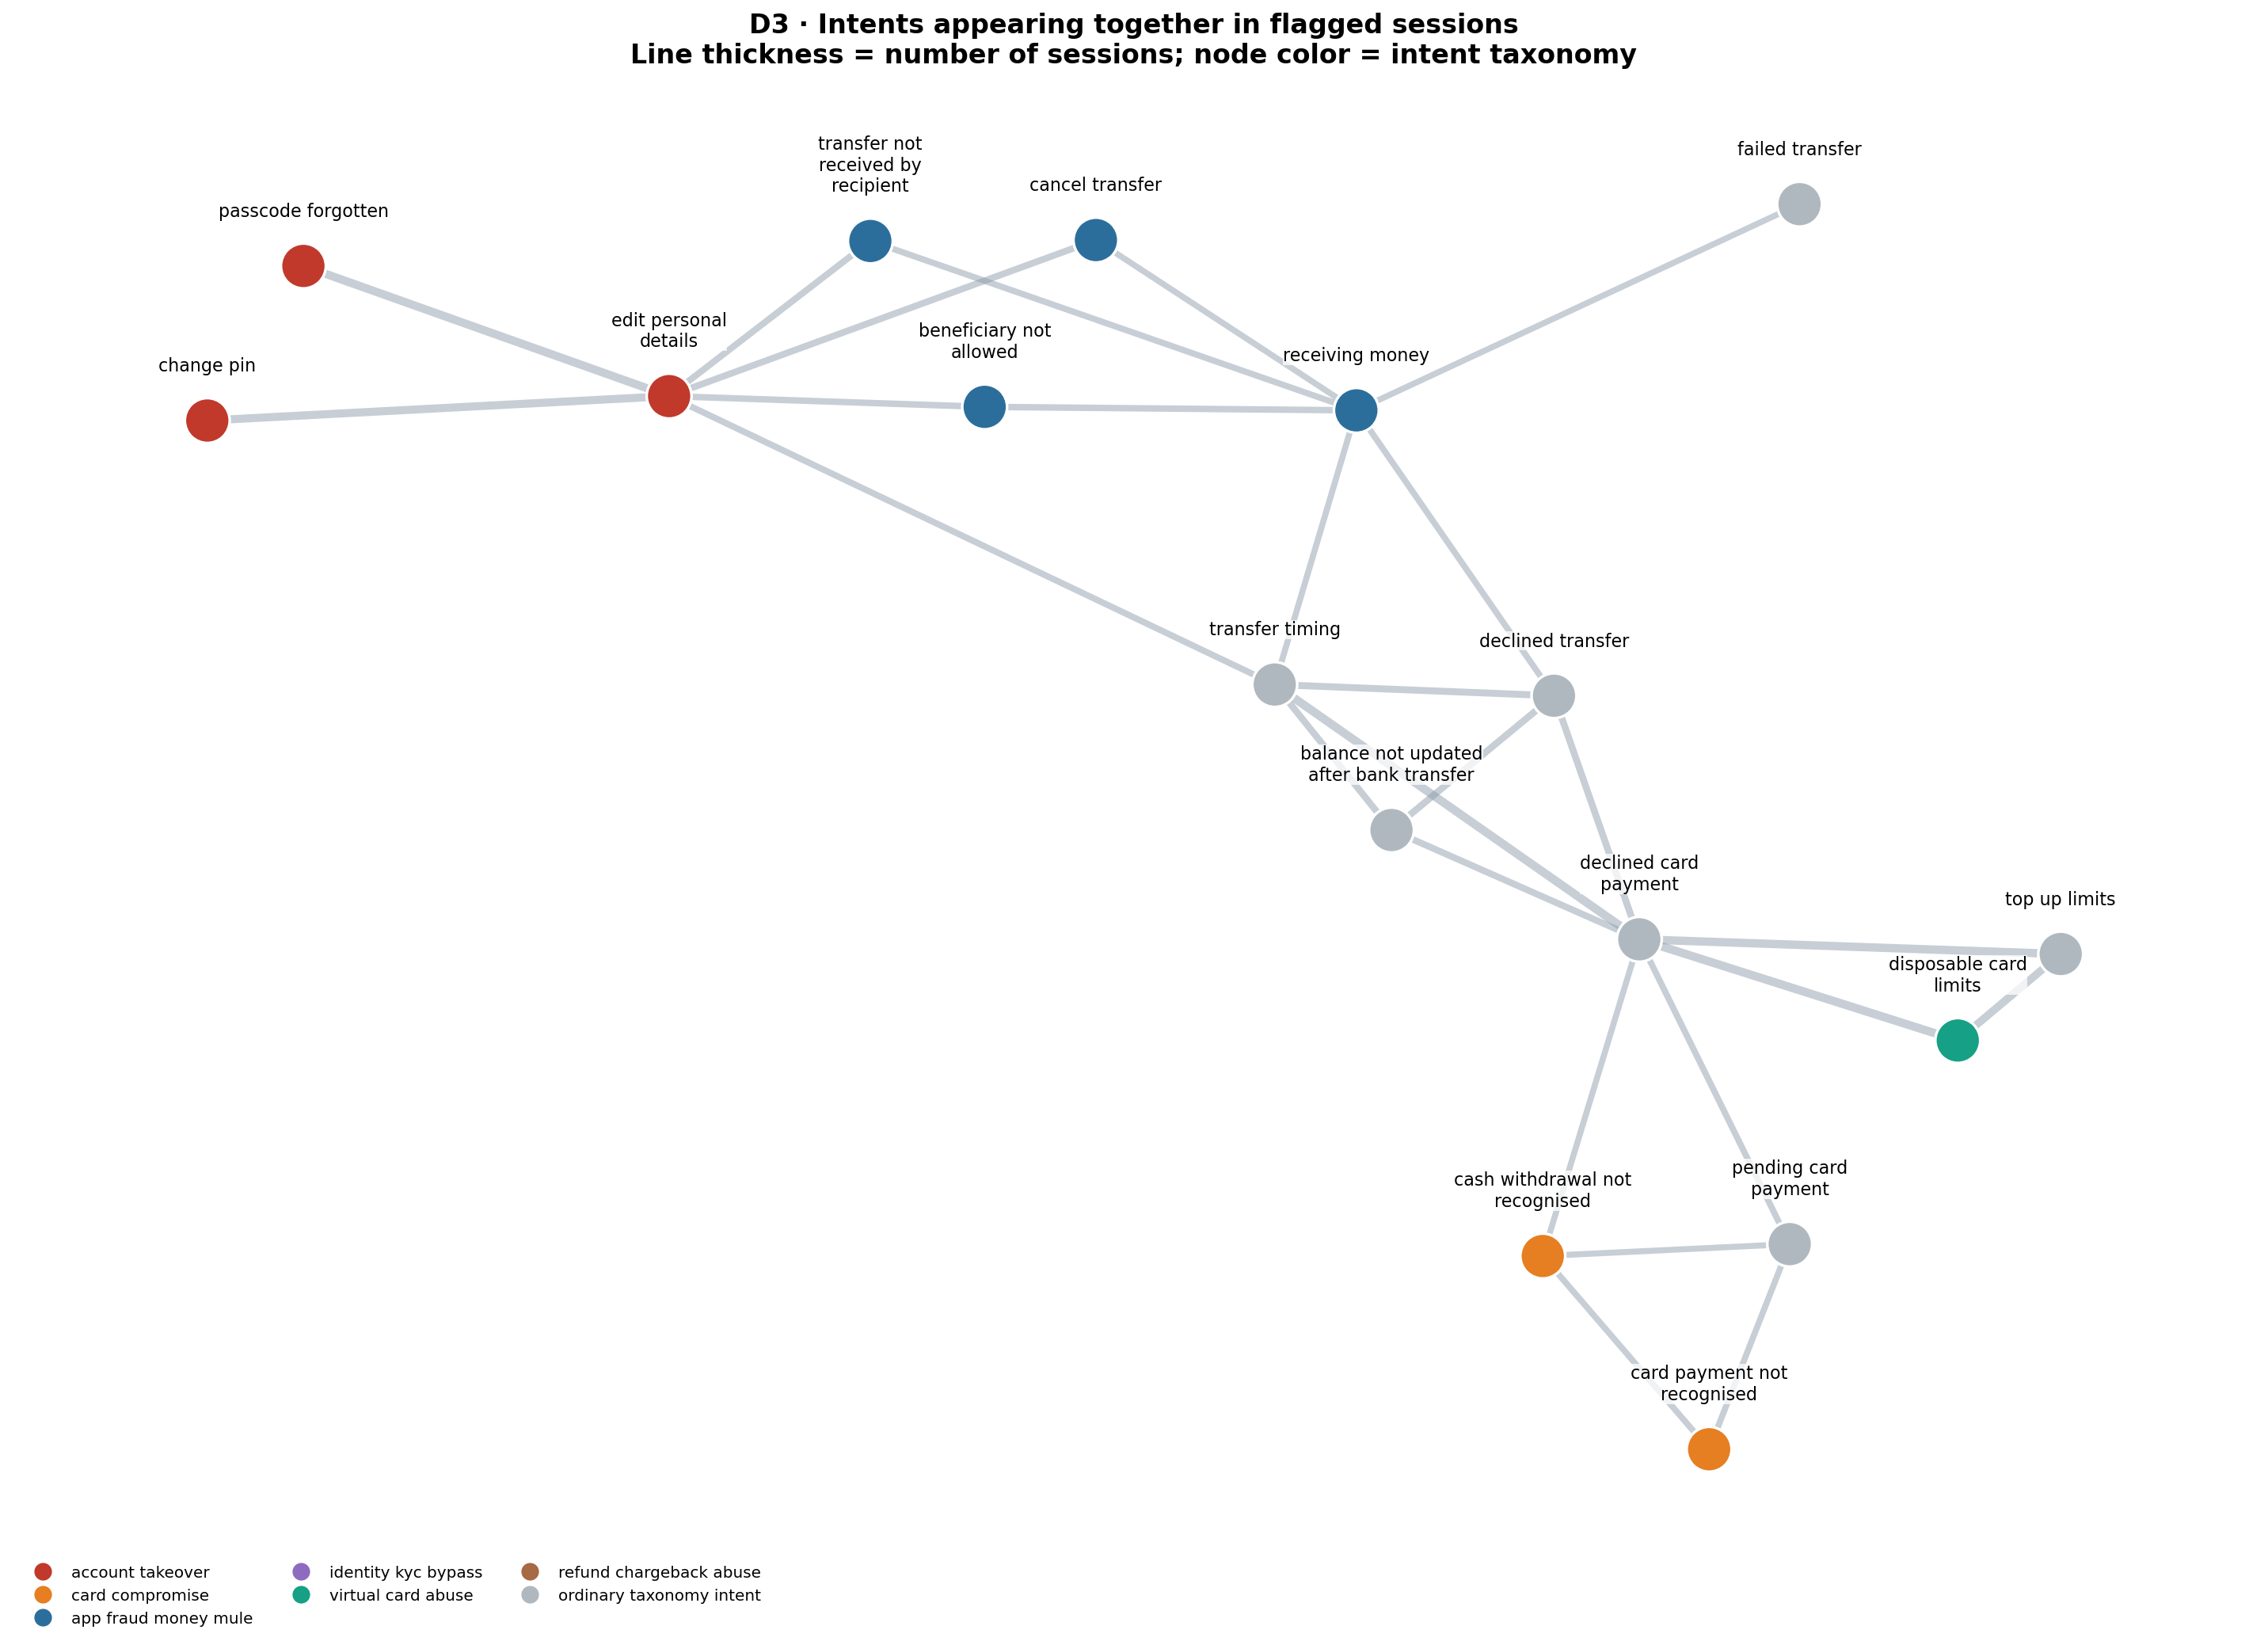
\includegraphics[keepaspectratio]{figures/D3_intent_cooccurrence_network.png}}

}

\caption{\label{fig-cooccurrence}Intent co-occurrence within flagged
development-stream sessions.}

\end{figure}%

\subsection{Implications for modeling}\label{implications-for-modeling}

The analyses motivate combining text with session size, duration, recent
message gaps, intent transitions, and location history. They also reveal
shortcuts a model might exploit. In the saved full-stream persona
summary, location-anomaly users average about 23 messages while normal
users average about 50; background volume therefore remains a potential
confound. These features require evaluation on held-out users or time
periods before they can support detection claims.

\section{Natural Language Processing}\label{sec-nlp}

\subsection{Text preparation and
TF-IDF}\label{text-preparation-and-tf-idf}

The scikit-learn baseline uses unigram/bigram TF-IDF with sublinear term
frequency, Unicode accent stripping, and a minimum document frequency of
two. The vectorizer is fitted on the original training split and
transforms the held-out test split.

The Spark pipeline lowercases and tokenizes text, constructs bigrams,
fits separate unigram and bigram count vocabularies with minimum
document frequency two, applies IDF weights, and assembles the vectors.
Its feature construction and regularization settings differ from the
scikit-learn pipeline; the reported scores are separate baseline results
rather than an isolated comparison of execution engines.

\subsection{Sentence embeddings and semantic
analysis}\label{sentence-embeddings-and-semantic-analysis}

Part A uses
\href{https://huggingface.co/sentence-transformers/all-MiniLM-L6-v2}{\texttt{all-MiniLM-L6-v2}}
to represent each message as a normalized 384-dimensional vector.
Fifteen cosine nearest neighbors characterize semantic overlap,
including an analysis excluding neighbors with the same intent. UMAP
uses cosine distance, fifteen neighbors, minimum distance 0.1, and
random seed 7 for visualization. These embeddings support EDA; they have
not been evaluated as features in the planned fraud comparison.

\subsection{Intent matching and
extensions}\label{intent-matching-and-extensions}

\section{Machine Learning}\label{sec-ml}

\subsection{Tasks and evaluation
design}\label{tasks-and-evaluation-design}

The completed supervised task predicts one of 77 intents using the
original 10,003/3,080 train/test split. The proposed fraud task instead
predicts simulated \texttt{is\_fraud}. Intent accuracy cannot substitute
for fraud precision or recall. Repeated training sentences in the
simulated stream also mean that scoring this stream is an operational
demonstration rather than an independent generalization benchmark.

\subsection{Intent classifiers}\label{intent-classifiers}

The scikit-learn model is logistic regression with \texttt{C=10}, up to
2,000 iterations, and random state 42. The Spark MLlib model is
multinomial logistic regression with \texttt{regParam=0.01}, no
elastic-net mixing, and up to 100 iterations. Its model is saved and
reloaded before scoring unlabeled messages. Predictions include the
assigned intent, taxonomy risk, probability-based confidence, and a
review flag when confidence is below 0.5. That threshold is a review
heuristic, not a calibrated fraud threshold.

The saved Spark intent notebook runs with \texttt{ON\_CLUSTER=False}. It
trains on the original Banking77 training split, not on the stream's
manually labeled subset; the stream is subsequently divided into labeled
and unlabeled tables for scoring.

\subsection{Text-only and text-plus-behavior fraud
models}\label{text-only-and-text-plus-behavior-fraud-models}

\section{Results}\label{sec-results}

\subsection{Intent classification}\label{intent-classification}

{\def\LTcaptype{none} % do not increment counter
\begin{longtable}[]{@{}lrrr@{}}
\toprule\noalign{}
Model & Test messages & Accuracy & Weighted F1 \\
\midrule\noalign{}
\endhead
\bottomrule\noalign{}
\endlastfoot
scikit-learn TF-IDF + logistic regression & 3,080 & 89.06\% & 89.08\% \\
Spark MLlib TF-IDF + logistic regression & 3,080 & 84.45\% & 84.49\% \\
\end{longtable}
}

Source: \texttt{eda/output/b1\_metrics.json} and
\texttt{spark/output/intent\_test\_metrics.csv}. The Spark result
additionally reports 85.17\% weighted precision and 84.45\% weighted
recall. Differences in pipeline settings prevent attributing the score
gap to distributed processing alone.

\subsection{Unlabeled stream scoring}\label{unlabeled-stream-scoring}

The saved local Spark run scores 350,036 unlabeled development-stream
messages. Mean reported confidence is 0.938; 0.90\% of predictions fall
below the review threshold, and 9.97\% receive an intent assigned medium
or high risk. These are prediction summaries, not fraud prevalence
estimates or held-out accuracy. The recorded training time is 49.1
seconds and scoring/write time is 9.3 seconds.

Source: \texttt{spark/output/intent\_scoring\_summary.csv} and
\texttt{intent\_timings.csv}.

\subsection{Contribution of behavior to fraud
detection}\label{contribution-of-behavior-to-fraud-detection}

\subsection{Full-stream distributed
processing}\label{full-stream-distributed-processing}

The saved S3/Spark run processes 50 million messages, one million users,
and 14,709,922 sessions across 365 days. Manual intent coverage is 30\%,
and the rounded simulated fraud-message rate is 1.29\%.

{\def\LTcaptype{none} % do not increment counter
\begin{longtable}[]{@{}lr@{}}
\toprule\noalign{}
Operation & Recorded time (seconds) \\
\midrule\noalign{}
\endhead
\bottomrule\noalign{}
\endlastfoot
Count raw stream & 319.8 \\
Compact daily files and rewrite user data & 560.9 \\
Count compacted stream & 10.0 \\
Full-stream overview & 32.7 \\
Daily aggregation & 13.0 \\
Message-gap quantiles using windows & 52.1 \\
Write session table & 74.5 \\
Summarize session table & 12.5 \\
\end{longtable}
}

Source: \texttt{spark/output/timings.csv}, \texttt{run\_summary.csv},
and \texttt{C1\_overview.csv}. Compaction reduces file count from 18,250
to 365 while preserving row count. The recorded counts differ by a
factor of about 32, but caching, metadata access, and run order are not
controlled, so this is not a general speedup benchmark.

\subsection{Full-stream session
summaries}\label{full-stream-session-summaries}

{\def\LTcaptype{none} % do not increment counter
\begin{longtable}[]{@{}
  >{\raggedright\arraybackslash}p{(\linewidth - 6\tabcolsep) * \real{0.2000}}
  >{\raggedleft\arraybackslash}p{(\linewidth - 6\tabcolsep) * \real{0.2667}}
  >{\raggedleft\arraybackslash}p{(\linewidth - 6\tabcolsep) * \real{0.2667}}
  >{\raggedleft\arraybackslash}p{(\linewidth - 6\tabcolsep) * \real{0.2667}}@{}}
\toprule\noalign{}
\begin{minipage}[b]{\linewidth}\raggedright
Message/session group
\end{minipage} & \begin{minipage}[b]{\linewidth}\raggedleft
Sessions
\end{minipage} & \begin{minipage}[b]{\linewidth}\raggedleft
Median messages
\end{minipage} & \begin{minipage}[b]{\linewidth}\raggedleft
Median duration (minutes)
\end{minipage} \\
\midrule\noalign{}
\endhead
\bottomrule\noalign{}
\endlastfoot
Ordinary & 14,629,922 & 3 & 6.0 \\
Account takeover & 19,927 & 6 & 16.7 \\
Money mule & 16,116 & 9 & 180.4 \\
Card testing & 16,127 & 11 & 16.4 \\
Location anomaly & 15,962 & 5 & 34.7 \\
Night activity & 11,868 & 9 & 95.9 \\
\end{longtable}
}

Source: \texttt{spark/output/C4\_session\_summary.csv}. These groups
describe ordinary sessions and flagged bursts, rather than assigning
every session from a fraud persona to fraud.

\subsection{Scope of performance
evidence}\label{scope-of-performance-evidence}

The repository demonstrates full-scale distributed analytics and a
separate local intent-model run. It does not provide controlled scaling
experiments, full-stream cluster intent inference, or measured
single-machine memory failure.

\section{Discussion and Conclusion}\label{sec-discussion}

\subsection{What the current results
establish}\label{what-the-current-results-establish}

Text models classify Banking77 intent with useful held-out accuracy,
while the routing and keyword analyses identify overlap between ordinary
and fraud-relevant wording. Spark processes the larger simulated stream
and extracts compact behavioral summaries. These results establish the
analysis foundation; they do not yet establish how much behavior adds to
fraud detection.

\subsection{Limitations and validity}\label{limitations-and-validity}

Fraud labels are assigned by generator rules. Learning those rules
successfully would not demonstrate performance on real bank fraud. User
histories, cities, and times are synthetic; city-center distances are
not verified impossible travel. Repeated source sentences limit
linguistic diversity. Taxonomy-assigned risk differs from simulated
message-level fraud, and false-alert rates measured against one
definition should not be described using the other.

Some background-volume differences and time-window restrictions could
provide artificial model shortcuts. The development EDA and full-scale
analytics also cover different date windows and populations; their
numbers should not be mixed. Probability confidence is not calibrated,
and the review threshold has not been validated against review capacity
or monetary costs.

\subsection{Future work}\label{future-work}

\subsection{Conclusion}\label{conclusion}

The project has implemented data cleaning, a reproducible simulated
message stream, text and behavioral EDA, intent classifiers, and
S3/Spark processing of 50 million messages. The strongest completed
predictive result is 89.06\% intent accuracy on the held-out Banking77
test split.

\section*{References}\label{sec-references}
\addcontentsline{toc}{section}{References}

\begin{itemize}
\tightlist
\item
  PolyAI.
  \href{https://huggingface.co/datasets/PolyAI/banking77}{Banking77
  dataset and dataset card}.
\item
  DSAN 6000. \href{https://jjacobs.me/dsan6000/final-project/}{Final
  Project: Datasets and Timeline}.
\item
  Sentence Transformers.
  \href{https://huggingface.co/sentence-transformers/all-MiniLM-L6-v2}{all-MiniLM-L6-v2
  model card}.
\item
  Project repository.
  \href{https://github.com/MingyangHan-1021/DSAN6000-Project}{Scalable
  Fraud Detection in Banking Chatbot Conversations}.
\end{itemize}

The implementation details and numerical results in this draft come from
the repository's scripts, executed notebooks, and saved tables
identified above.




\end{document}
